\documentclass[11pt,a4paper]{article}
\usepackage[top=3cm, bottom=2cm, left=3cm, right=2cm]{geometry}
\usepackage[utf8]{inputenc}
% \usepackage[T1]{fontenc}
\usepackage{amsmath, amsfonts, amssymb}
\usepackage{siunitx}
\usepackage[brazil]{babel}
\usepackage{graphicx}
\usepackage[margin=10pt,font={small, it},labelfont=bf, textfont=it]{caption}
\usepackage[dvipsnames, svgnames]{xcolor}
\DeclareCaptionFont{MediumOrchid}{\color[svgnames]{MediumOrchid}}
\usepackage[pdftex]{hyperref}
\usepackage{natbib}
\bibliographystyle{plainnat}
\bibpunct{[}{]}{,}{s}{}{}
\usepackage{color}
\usepackage{footnote}
\usepackage{setspace}
\usepackage{booktabs}
\usepackage{multirow}
\usepackage{subfigure}
\usepackage{fancyhdr}
\usepackage{leading}
\usepackage{indentfirst}
\usepackage{wrapfig}
\usepackage{mdframed}
\usepackage{etoolbox}
\usepackage[version=4]{mhchem}

\newcounter{exemplo}

\NewDocumentEnvironment{exemplo}{ O{} }{%
\allowbreak
\setlength{\parindent}{0pt}
  \begin{mdframed}[
  leftline=true,
  topline=false,
  rightline=false,
  bottomline=false,
  linewidth=2pt,
  linecolor=CarnationPink,
  frametitlerule=false,
  frametitlefont=\Large\bfseries\color{CarnationPink},
  frametitle={\color{CarnationPink}\normalfont\bfseries Exemplo: #1},
  ]
}{%
  \end{mdframed}
}

\setlength{\fboxsep}{10pt}
\setlength{\fboxrule}{1pt}
\usepackage{float}
\renewcommand{\thefootnote}{\alph{footnote}}
\usepackage{url}
\hypersetup{
    colorlinks=true,
    linkcolor=cyan,
    filecolor=cyan,      
    urlcolor=cyan,
    citecolor=cyan,
    pdftitle={Proteção Radiológica}
}
\pagestyle{fancy}
\fancyhf{}
\renewcommand{\headrulewidth}{0pt}
\rfoot{Página \thepage}
\title{Física Médica}
\author{Física Das Radiações\nocite{*}}
\date{\textit{Dalila Mendonça}}
\begin{document}
	\maketitle


    \section{Física Atômica e Nuclear}

        \subsection{Átomos}

            Um átomo é formado por um núcleo e uma eletrosfera. Os elétrons na eletrosfera que determinam as propriedades químicas dos átomos. Os elementos contidos no núcleo são chamados de núcleons, podendo ser ou próton ou nêutron. Os nuclídeos se referem a composição de prótons e nêutrons em um núcleo.

            Cada elemento, está relacionado com os seguintes números:

            \begin{itemize}
                \item \textbf{\textit{\textcolor{CarnationPink}{Z:}}} Número atômico. É definido como o número total de prótons de um elemento;
                \item \textbf{\textit{\textcolor{CarnationPink}{N:}}} Número total de nêutrons do elemento;
                \item \textbf{\textit{\textcolor{CarnationPink}{A:}}} Número de massa atômica, dado pela soma do número de prótons Z e o número de nêutrons N de um material (A = Z + N);
            \end{itemize}
            
            Ao avaliar diferentes nuclídeos, eles podem ser classificados como:

            \begin{itemize}
                \item \textbf{\textit{\textcolor{CarnationPink}{Isótopo}}}: São aqueles elementos que possuem o mesmo número de prótons mas diferentes números de nêutrons, ou seja, possuem as mesmas propriedades químicas, mesmo número atômico mas diferênte número de massa e diferente propriedade relacionada decaimento nuclear Ex:  $ {}_{53}^{125} \mathbf{I} $ e $ {}_{53}^{131} \mathbf{I} $
                \item \textbf{\textit{\textcolor{CarnationPink}{Isótono}}}: São aqueles elementos que possuem o mesmo número de nêutrons mas número de prótons diferentes. Este tipo de classificação raramente é utilizada;
                \item \textbf{\textit{\textcolor{CarnationPink}{Isóbaro}}}: São aqueles elementos que possuem o mesmo número de nucleons, ou seja, o mesmo número de massa, mas se trata de diferentes nuclídeos, ou seja, quantidades diferentes de prótons e nêutrons. O decaimento beta e a captura eletrônica resulta em um isóbaro. Ex. O ${}^{131} \mathbf{I}$ decai para o ${}^{131} \mathbf{Xe}$.
                \item \textbf{\textit{\textcolor{CarnationPink}{Isômero}}}: Se trata do mesmo nuclídeo, ou seja, mesmo número de massa e número atômico, mas se encontram em diferentes estados de energia (estado excitado ou não-excitado). Ex. O ${}^{99m} \mathbf{Tc}$ decai para o ${}^{99} \mathbf{Tc}$ emitindo radiação $\gamma$ sem alterar seu número de prótons ou nêutrons.
            \end{itemize}

        
            \subsubsection{Forças Fundamentais}

                As forças fundamentais encontradas na natureza são: Força Forte, Força eletromagnética, Força Fraca e a Força Gravitacional, onde:

                \begin{itemize}
                    \item \textbf{\textit{\textcolor{CarnationPink}{Força Nuclear Forte}}}: É a maior força encontrada na natureza; É responsável por manter o núcleo unido, contendo a repulsão Coulombiana entre os prótons do núcleo.
                    \item \textbf{\textit{\textcolor{CarnationPink}{Força Eletromagnética}}}: Equivale a 1/100 da força forte. É a força que atua entre partículas carregadas, onde partículas com mesma carga se repelem entre si enquanto que partículas com cargas diferentes se atraem entre si.
                    \item \textbf{\textit{\textcolor{CarnationPink}{Força Nuclear Fraca}}}: Equivale a 1/1000000 da força forte. É a força que une os quarks para formar os nucleons e está relacionada ao decaimento radioativo. Ex. o \textsuperscript{14}\textbf{C} decai para o  \textsuperscript{14}\textbf{N} a partir da transformação de um próton em um nêutron emitindo uma partícula $\beta ^-$; esta transformação só é possível graças a força nuclear Fraca.
                    \item \textbf{\textit{\textcolor{CarnationPink}{Força Gravitacional}}}: Equivale a ~$1 \times 10^{-39}$ da Força Forte e não tem relevância na escala atômica.
                \end{itemize}

        \subsection{Núcleo}
            \subsubsection{Equivalência de Massa e Energia}

                E equação  $E = m c^2$ permite a conversão entre massa e energia pelo fator $c^2$, isso diz que quando as partículas se aproximam da velocidade da luz, a velocidade se tornará constante de forma que caso a partícula ganhe energia, ela na verdade ganhará massa.


                \begin{itemize}
                    \item \textbf{\textit{\textcolor{CarnationPink}{Unidade de Massa atômica (u):}}}Definida como 1/12 da massa do Carbono-12. É ligeiramente menor que a soma das massas dos componentes do átomo devido a quantidade de massa convertida em energia de ligação do átomo de Carbono-12.  
                    \item \textbf{\textit{\textcolor{CarnationPink}{Energia Equivalente:}}} É definida como a quantidade de energia equivalente, dada em \unit{MeV/c^2}:

                \end{itemize}

            
            \begin{table}[h]
                \centering
                \caption{Valores de massa para as partículas que compõem o átomo onde 1 u = 931.5 \unit{MeV/c^2}}
                \begin{tabular}{c c c}
                    \toprule
                    Partícula &  u & \unit{MeV/c^2} \\
                    \midrule
                    Prótons & 1.00728 & 938.3 \\
                    Nêutrons & 1.00866 & 939.6 \\
                    Elétrons & 0.0005 & 0.511\\
                    \bottomrule
                    \bottomrule
                \end{tabular}
            \end{table}

            
            Algumas relações importantes:

            \begin{itemize}
                \item \textbf{\textit{\textcolor{CarnationPink}{Grama-átomo}}}: O número de massa atômica A de todos os elementos é definido de forma que em A gramas de um determinado  elemento contenha exatamente $N_A = 6.022 \times 10^{23}$ átomos desse elemento. Por exemplo, e 1g-átomo de \textsuperscript{60}C existem 60g de \textsuperscript{60}C; E em 60 g de \textsuperscript{60}C existem $6.022 \times 10^{23}$ átomos de \textsuperscript{60}C.
                
                \item \textbf{\textit{\textcolor{CarnationPink}{Número de átomos por massa de um elemento:}}} É obtido através da relação:
                    \begin{equation}
                        N_a = N_A \frac{m}{A} 
                    \end{equation}
                    

                \item \textbf{\textit{\textcolor{CarnationPink}{Número de elétrons por massa de um elemento:}}} é obtido através da relação:
                    \begin{equation}
                        N_e = Z \frac{N_a}{m} =  \frac{Z}{A} N_A
                    \end{equation}
                    

                \item \textbf{\textit{\textcolor{CarnationPink}{Número de elétrons por volume de um elemento:}}} é obtido através da relação:
                    
                    \begin{equation}
                        N_e^V = Z \frac{N_A}{V} = \rho Z \frac{N_a}{m} = \rho Z \frac{N_A}{A}
                    \end{equation}
                    
            \end{itemize}
              
            \subsubsection{Raio do Núcleo}

                O raio de núcleo r pode ser estimado a partir da relação:

                \begin{equation}
                    r = r_0 \sqrt[3]{A} 
                \end{equation}

                onde $r_0$ é uma constante igual a 1/2 do raio clássico do elétron, sendo o raio do elétron:

                \begin{equation}
                    r_e = \frac{e^2}{4 \pi \epsilon_0 m_e c^2} = 2.818 \; fm
                \end{equation}
            
            \subsubsection{Energia de Ligação Nuclear}

                Quando as partículas são ligadas umas às outras para formar o núcleo, elas cedem parte da sua massa que é convertida em energia de ligação das partículas ao núcleo. Em outras palavras, a energia de ligação nuclear e a energia necessária para ligar os prótons e nêutrons no núcleo. 

                Este processo resulta em um déficit de massa, caracterizado pela diferença de massa entre a soma dos nucleons separadamente e a massa do núcleo em si. Esse déficit de massa é equivalente, então, à energia de ligação nuclear.

                O déficit de massa é obtido através da Equação:

                    \begin{equation}
                        \Delta  m = Zm_p + (A - Z)m_n - M
                    \end{equation}

                onde $m_p$ é a massa do próton, $m_n$ é a massa do nêutron e M é a massa atômica do elemento.

                A energia de ligação nuclear é então:

                    \begin{equation}
                        E_B = \Delta m \cdot c^2
                    \end{equation}

                
                \begin{exemplo}[Déficit de Massa do \textsuperscript{12}C]
                    
                    O Carbono-12 contém 6 prótons e 6 nêutrons. 
                    
                    A soma total da massa dos prótons é de:

                    $$m_p = 6 \times 1.00728 \; amu = 6.04368 \; amu$$

                    A soma total da massa dos nêutrons é de:

                    $$m_n = 6 \times 1.00866 \; amu = 6.05196 \; amu$$

                    A soma de todos os componentes será então de: 

                    $$soma = 6.04368 + 6.05196 \thickapprox  12.0956 \; amu$$

                    Porém a massa do Carbono-12 é de 12.000 amu, e portanto o déficit de massa:

                    $$12.0956 - 12 = 0.0956 \; amu = 0.956 \times 931.5 \; Mev \thickapprox 89 \;  MeV$$ 

                    é a energia necessária para manter o núcleo do Carbono-12 ligado.
                \end{exemplo}

                Portanto, para separar um núcleo de Carbono-12 seriam necessários fornecer no mínimo 89 MeV de energia. Um fóton produzido em um acelerador clínico com energia de até 18MV não conseguiria separar um núcleo de C-12, já um próton acelerado em um ciclotron com energia de até 200 MeV teria esta capacidade. 
        
            \subsubsection{Estabilidade Nuclear}
                
                A estabilidade nuclear está relacionada a quantidade de prótons e nêutrons dentro do núcleo; Quanto maior o número de prótons em um núcleo, maior a repulsão coulombiana e então mais nêutrons são necessários para afastar os prótons um do outro 
                (Lembrando que a força eletromagnética diminui com o inverso do quadrado da distância). Portanto o excesso de prótons ou nêutrons no núcleo leva a instabilidade nuclear.
                
                Os núcleos instáveis decaem para nucleos menos instáveis, cujo modo de decaimento depende da razão entre o número de nêutrons e o número de prótons deste núcleo. 

                \begin{itemize}
                    \item Para núcleos com Z até 20 (Cálcio - Ca) a razão mágica n/p relacionada aos núcleos estáveis é de 1:1;
                    \item Para nucleos com Z acima de 20, a razão mágica é maior que 1:1; Por exemplo o Ouro-197 (\textsuperscript{197}Au)  possui n = 118 e p = 79, ~ 1.5:1;
                \end{itemize}

                A Figura \ref{fig:estabilidadeNuclear} mostra a curva de dos núcleos estáveis comparado com a razão n/p = 1; Nota-se que com o aumento do número de prótons é necessário um aumento no número de nêutrons para manter a estabilidade nuclear. O Bismuto (Z = 83) é o núcleo estável mais pesado, qualquer núcleo acima dele é instável.

                \begin{figure}[h]
                    \centering
                    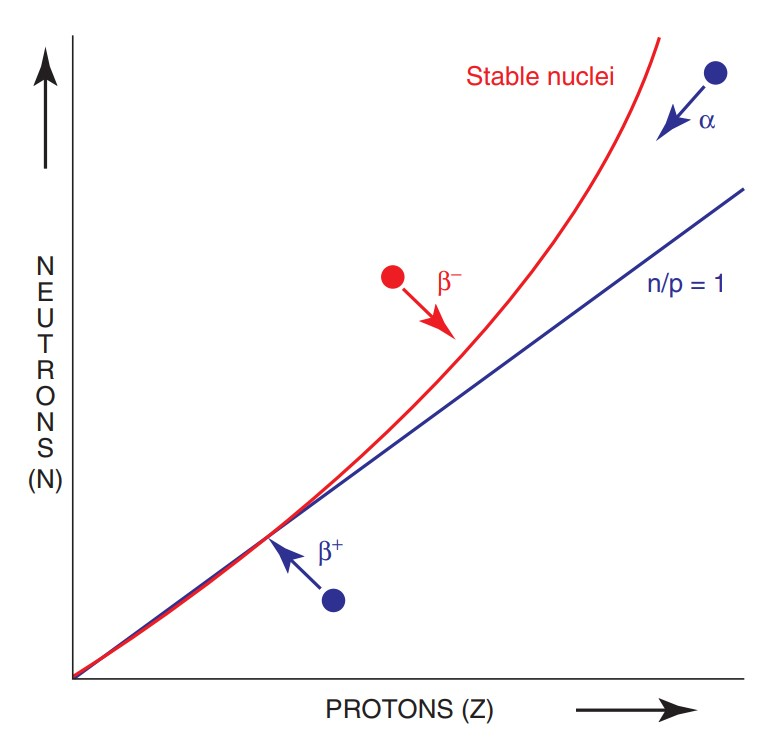
\includegraphics[width=0.7\textwidth]{Imagens/graficoNucleosEstaveis.jpg}
                    \caption{Estabilidade Nuclear, onde a linha vermelha representa os núcleos estáveis.}
                    \label{fig:estabilidadeNuclear}
                \end{figure}
        
            \subsubsection{Energia de Ligação Por Núcleon}
                
                A medida que o número atômico aumenta, a força forte aumenta e então a energia de ligação nuclear aumenta lentamente até um certo limiar, Z $<$ 26 (Ferro - Fe). A partir deste limiar, a força repulsiva entre os prótons começa a se sobressair e portanto, mesmo que a energia de ligação nuclear total continue aumentando, a energia de ligação por núcleons começa a diminuir; O maior valor possível para a energia de ligação por núcleon é de  \qty{8.7}{MeV}, que ocorre para A $\approx$ 60. A $E_B$ é da ordem de $\thicksim$ \qty{8}{MeV/nucleon} e é necessário no mínimo \qty{8.6}{MeV/nucleon} para que o núcleo seja estável.

                Quando os átomos estão instáveis, a força fraca permite a transformação dos núcleons, por exemplo um prótons se transformar em um nêutron no processo de decaimento. Os núcleos pesados, com Z $>$ 52  (Telúrio) podem ser quebrados em pedaços maiores, normalmente em pares como a partícula-$\alpha$ (${}_2^4He$).
                
                A energia de ligação por nucleon pode ser obtida através da relação:

                    \begin{equation}
                        E_{Bnucleon} = \frac{E_B}{Nucleon} = \frac{\Delta m c^2}{A} = \frac{\left[Zm_p + (A - Z)m_n - M\right]c^2}{A}
                    \end{equation}

            \subsubsection{Emparelhamento dos Nucleons}

                Geralmente núcleons pares são mais estáveis que os núcleons ímpares, ou seja, ter um número par de prótons e um número par de nêutrons e por essa razão, núcleos mais pesados tendem a emitir pares de partículas ao invés emitir nêutrons ou prótons isoladamente. Ainda é possível encontrar poucos núcleos estáveis com números pares de prótons e impares de nêutrons e vice-versa, porém existem apenas 4 elementos estáveis com números impares de prótons e nêutrons, sendo eles: 

                \begin{enumerate}
                    \item \textbf{\textsuperscript{2}H:} Deutério, contendo 1p e 1n;
                    \item \textbf{\textsuperscript{6}Li:} Lítio-6, contendo 3p e 3n;
                    \item \textbf{\textsuperscript{10}B:} Boro-10, contendo 5p e 5n; e 
                    \item \textbf{\textsuperscript{14}N:} Nitrogênio-14; contendo 7p e 7n;
                \end{enumerate}

                \textbf{\textcolor{CarnationPink}{\textit{Obs:}}} O Boro-10 é um elemento utilizado no tratamento de câncer utilizando captura de nêutrons, onde o \textsuperscript{10}B é incorporado à compostos com afinidade à tecidos cancerígenos que são injetados nos pacientes.Quando estes compostos entram em contato com nêutrons de alta energia, capturam esses nêutrons liberando partículas carregadas que destroem as células onde estão inseridos.


            \subsubsection{Modelos Nucleares}
                
                Existem vários modelos nucleares que foram propostos para descrever a estrutura do núcleo atômico. Alguns dos modelos mais importantes são:

                \begin{itemize}

                    \item Modelo de gotas: Este modelo descreve o núcleo como uma esfera de matéria líquida, na qual os prótons e nêutrons estão distribuídos de forma uniforme. Este modelo é capaz de explicar algumas propriedades do núcleo, como a energia de ligação, mas falha em explicar outras propriedades, como a distribuição das energias dos níveis de energia.
                    
                    \item Modelo de camadas: Este modelo descreve o núcleo como uma série de camadas de prótons e nêutrons, semelhante à estrutura do modelo atômico de Bohr. Este modelo é capaz de explicar algumas propriedades do núcleo, como as energias dos níveis de energia, mas não é capaz de explicar a natureza da interação forte, que mantém o núcleo unido.
                    
                    \item Modelo de quarks: Este modelo descreve o núcleo como um conjunto de quarks, que são as partículas fundamentais que compõem prótons e nêutrons. Este modelo é capaz de explicar algumas propriedades do núcleo, como a distribuição de massa e as energias dos níveis de energia, mas ainda não é completamente compreendido.
                    
                    \item Modelo de shell: Este modelo é uma extensão do modelo de camadas, que descreve o núcleo como uma série de camadas de prótons e nêutrons, com um número específico de partículas em cada camada. Este modelo é capaz de explicar muitas propriedades do núcleo, como as energias dos níveis de energia e a distribuição de massa, e é amplamente utilizado na física nuclear.
                \end{itemize}

                Cada um desses modelos descreve a estrutura do núcleo de uma maneira diferente, e cada um contribuiu para a nossa compreensão atual da estrutura nuclear. O modelo de shell é o mais utilizado atualmente para descrever a estrutura do núcleo.

            \subsubsection{Reações Nucleares}
                
                Quando um nuclídeo $A$ é bombardeado com uma partícula $a$, podem ocorrer 3 tipos de interações:

                \begin{enumerate}
                    \item Espalhamento Elástico: Quando nenhuma energia é transferida da partícula $a$ para o nuclídeo $A$, porém o projétil muda sua trajetória;
                    \item Espalhamento Inelástico: Quando a partícula $a$ entra no núcleo de $A$ e é re-emitida com uma energia menor em uma direção diferente da direção de incidência; e   
                    \item Reação Nuclear: Quando a partícula $a$ entra no núcleo de $A$ e o transforma em um nuclídeo $B$ emitindo uma partícula $b$ diferente da partícula incidente $a$. 
                \end{enumerate}

                A Reação Nuclear é um  processo em que há conservação de carga, massa-energia, momento linear e número de massa. Uma reação nuclear pode ser descrita das seguintes formas:
                    
                    \begin{equation}
                        a + A \rightarrow B + b \qquad ou \qquad A(a, b)B
                    \end{equation}
                
                Para ocorrer uma reação nuclear é necessário um limiar de energia cinética para a partícula incidente, abaixo do qual uma reação nuclear não será desencadeada. Esta energia pode ser obtida através das equações de conservação de energia e momento relativísticas, sendo então:

                    \begin{equation}
                        E_k^{min} = \frac{\left(m_B \; c^2 + m_b \; c^2\right)^2 - \left(m_A \; c^2 + m_a \; c^2\right)^2}{2m_A \; c^2}
                    \end{equation}

        \subsection{Modelos Atômicos}

            Os modelos atômicos foram desenvolvidos no decorrer do tempo, sendo eles:
            
            \begin{itemize}
                \item \textbf{\textit{\textcolor{CarnationPink}{Modelo Atômico de Dalton:}}}
            \end{itemize}

                Este modelo foi proposto por John Dalton em 1808 e postula que os átomos são esferas rígidas e indivisíveis, que se combinam em proporções inteiras para formar compostos, mas falhou em explicar a existência de isótopos e de compostos moleculares.

            \begin{itemize}
                \item \textbf{\textit{\textcolor{CarnationPink}{Modelo Atômico de Thomson:}}}
            \end{itemize}

                Este modelo foi proposto por J.J. Thomson em 1897 e postula que os átomos são esferas carregadas positivamente, com elétrons negativos incrustados na esfera, como passas em um pudim, mas não explicou como os elétrons estavam dispostos na esfera e como se organizavam para formar as ligações químicas.

            \begin{itemize}
                \item \textbf{\textit{\textcolor{CarnationPink}{Modelo Atômico de Rutherford:}}}
            \end{itemize}

                Este modelo foi proposto por Ernest Rutherford em 1911 e postula que os átomos consistem em um pequeno núcleo denso e carregado positivamente, cercado por elétrons orbitando o núcleo, mas não explicou por que os elétrons não caíam em direção ao núcleo devido à atração eletrostática.

            \begin{itemize}
                \item \textbf{\textit{\textcolor{CarnationPink}{Modelo Atômico de Bohr:}}}
            \end{itemize}

                Este modelo foi proposto por Niels Bohr em 1913 e postula que os elétrons orbitam o núcleo em órbitas quantizadas, e só podem existir em determinados níveis de energia. Este modelo descreveu a estrutura dos átomos de hidrogênio como elétrons em órbitas fixas, mas não explicou a estrutura de átomos maiores ou de moléculas.

            \begin{itemize}
                \item \textbf{\textit{\textcolor{CarnationPink}{Modelo Atômico de Sommerfeld:}}}
            \end{itemize}

                Este modelo foi proposto por Arnold Sommerfeld em 1916 e é uma extensão do modelo de Bohr, que permite que os elétrons existam em órbitas elípticas, bem como em níveis de energia mais elevados. Este modelo melhorou o modelo de Bohr ao incluir órbitas elípticas e subníveis, mas não explicou a natureza da mecânica quântica.


            \begin{itemize}
                \item \textbf{\textit{\textcolor{CarnationPink}{Modelo Atômico Quântico-Mecânico:}}}
            \end{itemize}

                Este modelo foi desenvolvido na década de 1920 por vários físicos, incluindo Louis de Broglie, Werner Heisenberg, Erwin Schrödinger e Max Born, e descreve os elétrons como ondas de probabilidade que ocupam regiões de espaço conhecidas como orbitais. Este modelo é a descrição mais atual da estrutura atômica, mas ainda existem limitações, como a dificuldade em visualizar os elétrons como partículas e a natureza probabilística dos elétrons.
        
            \subsubsection{Modelo Atômico de Rutherford}

                Foi um modelo baseado nos resultados de um experimento que buscava validar o modelo atômico de Thompson, que dizia que as cargas positivas e negativas estavam uniformemente distribuídas em um volume atômico esférico. Porém os experimêntos levaram a conclusão de que as cargas positivas e a maior parte da massa do átomo estava concentrada no núcleo do átomo e que as cargas negativas estavam espalhadas nas periferias do átomo. 

            \subsubsection{Modelo Atômico de Bohr}

                É o modelo clássico para o átomo que funciona bem para descrever um átomo de hidrogênio ou aqueles átomos que possuem apenas um elétron orbital, como o Hélio ionizado ou o lítio duplamente ionizado. Este modelo expandiu o modelo atômico de Rutherford combinando a mecânica clássica e a mecânica não-relativística juntamente com o conceito de momento angular quantizado para descrever a forma com o qual os elétrons se comportam no átomo, Figura \ref{fig:modeloAtomicoDeBohr}.

                \begin{figure}[h]
                    \centering
                    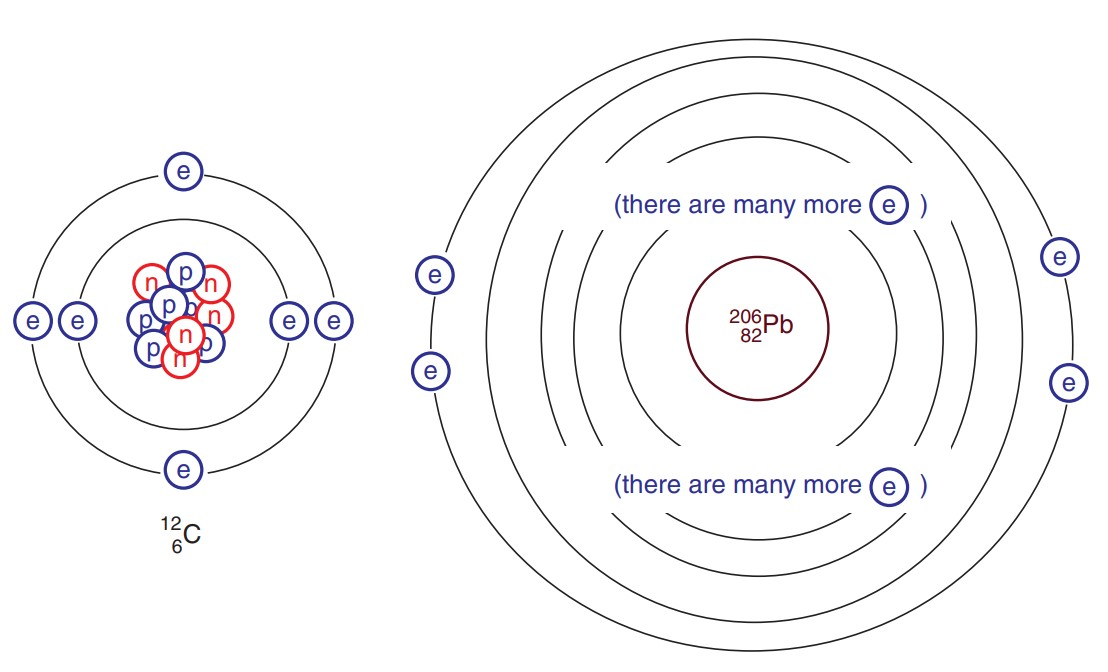
\includegraphics[width=0.7\textwidth]{Imagens/modeloAtomicoDeBohr.jpg}
                    \caption{Modelo Atômico de Bohr. Pode-se observar que quanto maior Z, maior o raio do átomo. A medida que os elétrons são adicionados, eles preenchem as camadas de maior energia, mais distantes do núcleo, em caminhos fixos}
                    \label{fig:modeloAtomicoDeBohr}
                \end{figure}

            \subsubsection{Raio Atômico de Bohr}

                O raio atômico de Bohr é uma medida teórica do tamanho do átomo, proposta por Niels Bohr em 1913. Ele calculou o raio do átomo de hidrogênio em seu estado fundamental (ou seja, com apenas um elétron) usando a teoria do modelo atômico de Bohr é definido como a distância média entre o elétron e o núcleo em uma órbita estacionária do átomo de hidrogênio em seu estado fundamental. 

                O raio atômico de Bohr é obtido através da Equação \ref{eq:raioAtomicoDeBohr}:

                \begin{equation}
                    a_0 = \frac{\hslash \; c}{\alpha \; m_e \; c^2}
                    \label{eq:raioAtomicoDeBohr}
                \end{equation}

                onde:

                $$\alpha = \frac{e^2}{4 \pi \epsilon_0} \; \frac{1}{\hslash c} = \frac{1}{137}$$


                O que nos permite reescrever a equação \ref{eq:raioAtomicoDeBohr}, chegando no valor para o raio atômico de Bohr:

                $$a_0 = \frac{4 \pi \epsilon_0}{e^2} \; \frac{(\hslash c)^2}{m_e \; c^2} = 0.5292 \mathring{A} $$

            \subsubsection{Os Postulados do Modelo atômico de Bohr}

                O modelo atômico de Bohr se baseia em 4 postulados:

                \begin{enumerate}
                    \item Postulado: Os elétrons giram em torno do núcleo de Rutherford em orbitas permitidas bem definidas (camadas). A força de atração Coulombiana $$F_{coul} = \frac{Ze^2 }{4 \pi \epsilon_0 r^2}$$ entre as cargas positivas no núcleo e os elétrons orbitais é equilibrada pela força centrífuga $$F_{cent} = \frac{m_e v^2}{r}$$ onde Z é o número de prótons no núcleo, r é o raio da órbita, m\textsubscript{e} é a massa do elétron e  v é a velocidade do elétron na órbita.
                    
                    \item Postulado: Uma vez em órbita, o elétron não perde nenhuma energia mesmo sendo constantemente acelerado; O que viola uma lei básica da natureza que diz que partículas carregadas aceleradas perderão parte de sua energia em forma de radiação;
                    
                    \item Postulado: Uma vez que o momento angular é uma grandeza física que descreve a rotação de um objeto ao redor de um eixo dado pela combinação do momento de inércia do objeto e sua velocidade angular em torno desse eixo; O momento angular $$L = m_e v r$$ de um elétron em uma órbita permitida é quantizado e dado por $$L = n \hslash$$ onde n é um número inteiro que se refere ao número quântico principal e $\hslash = h / 2 \pi$ onde h é a constante de Planck. A quantização simples do momento angular estipula que o momento angular pode ter apenas múltiplos inteiros de $\hslash$
                    
                    \item Postulado: Um átomo ou íon emite radiação quando um elétron faz uma transição de uma órbita com o número quantico inicial n\textsubscript{i} para uma órbita com o número quantico final n\textsubscript{f} para n\textsubscript{i} $>$ n\textsubscript{f}.
                \end{enumerate}

                O raio r\textsubscript{n} de um átomo de Bohr com um único elétron é dado pela  relação:

                    \begin{equation}
                        r_n = a_0 \left(\frac{n^2}{Z}\right) = 0.529 \mathring{A} \left(\frac{n^2}{Z}\right)
                    \end{equation}

                Onde $a_0$ é o raio de Bohr.

                A velocidade $v_n$ de um elétron em um átomo de Bohr monoeletrônico é dada pela equação:

                    \begin{equation}
                        v_n  = \alpha c \left(\frac{Z}{n}\right) = \frac{c}{137}\left(\frac{Z}{n}\right)
                    \end{equation}

                Os níveis de energia para as camadas orbitais dos elétrons em átomos monoeletrônicos são obtidos através da relação:

                    \begin{equation}
                        E_n = -E_R \left(\frac{Z}{n}\right)^2 = -13.6 \; eV \left(\frac{Z}{n}\right)^2
                    \end{equation}

                \noindent onde $E_R$ é a energia de Rydberg, $n$ é  o número quântico principal (se n = 1 então átomo está no seu estado fundamental, se n > 1 o átomo está em um estado excitado) e $Z$ é o número atômico (Z = 1 para o hidrogênio, Z = 2 para o Hélio com 1 ionização e Z = 3 para o Lítio com duas ionizações.) 
            
            \subsubsection{Espectro de Emissão Para o Átomo de Hidrogênio}

                As séries para o átomo de hidrogênio são sequências de transições eletrônicas que ocorrem quando um elétron é excitado e se move de um nível de energia mais alto para um nível de energia mais baixo, liberando energia na forma de luz. A Figura \ref{fig:diagramaNiveisDeEnergiaParaOAtomoDeHidrogenio} mostra o diagrama para os níveis de energia do átomo de hidrogênio. 

                    \begin{figure}[h]
                        \centering
                        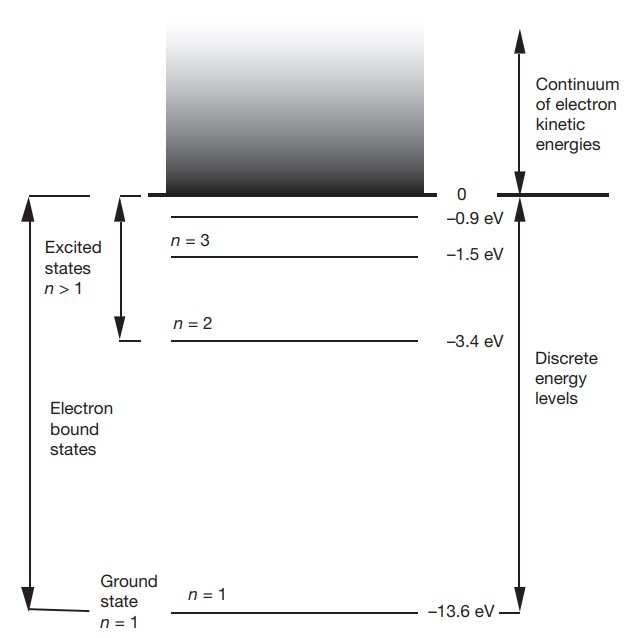
\includegraphics[width=0.7\textwidth]{Imagens/diagramaNiveisDeEnergiaParaOAtomoDeHidrogenio.jpg}
                        \caption{Diagrama dos níveis de energia para o átomo de hidrogênio}
                        \label{fig:diagramaNiveisDeEnergiaParaOAtomoDeHidrogenio}
                    \end{figure}

                As séries espectrais mais conhecidas são:

                \begin{itemize}

                    \item Série de Lyman: Esta série ocorre quando um elétron se move do nível n $\geqslant $ 2 para o nível n = 1, liberando energia na forma de luz ultravioleta.
                
                    \item Série de Balmer: Esta série ocorre quando um elétron se move do nível n $\geqslant $ 3 para o nível n = 2, liberando energia na forma de luz visível (especificamente, luz de comprimento de onda correspondente a linhas espectrais do espectro de Balmer).
                
                    \item Série de Paschen: Esta série ocorre quando um elétron se move do nível n $\geqslant $ 4 para o nível n = 3, liberando energia na forma de luz infravermelha.
                
                    \item Série de Brackett: Esta série ocorre quando um elétron se move do nível n $\geqslant $ 5 para o nível n = 4, liberando energia na forma de luz infravermelha de comprimento de onda mais longo do que a série de Paschen.
                
                    \item Série de Pfund: Esta série ocorre quando um elétron se move do nível n $\geqslant $ 6 para o nível n = 5, liberando energia na forma de luz infravermelha de comprimento de onda mais longo do que a série de Brackett.
                \end{itemize}

                Cada série é caracterizada por um conjunto específico de comprimentos de onda de luz liberada e tem um papel importante na espectroscopia e na compreensão da estrutura atômica.

            

        \subsection{Átomos com Multielétrons}
            
            Até então foram abordados os comportamentos para átomos com apenas um elétron orbital, porém para átomos com mais de um elétron alguns comportamentos são acrescentados. A Figura \ref{fig:diagramaNiveisDeEnergiaParaAtomosMultieletrons} mostra os níveis de energia para um átomo de chumbo, que se assemelha ao espectro do átomo de hidrogênio exceto pela quantidade de elétrons em cada camada e a maior energia de ligação nas camadas mais internas do átomo.

                \begin{figure}[h]
                    \centering
                    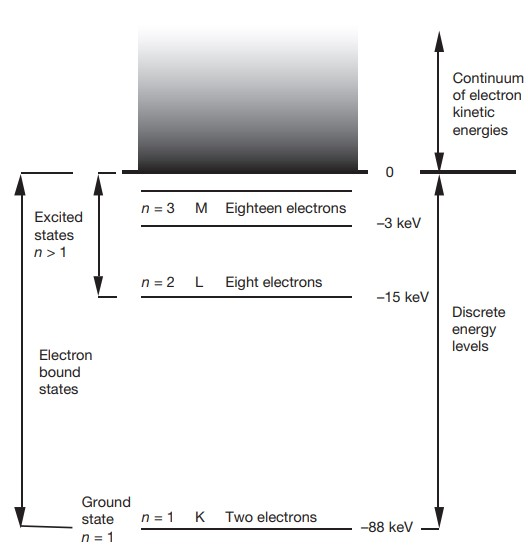
\includegraphics[width=0.7\textwidth]{Imagens/diagramaNiveisDeEnergiaParaAtomosMultieletrons.jpg}
                    \caption{Diagrama dos níveis de energia para um átomo de chumbo}
                    \label{fig:diagramaNiveisDeEnergiaParaAtomosMultieletrons}
                \end{figure}

            \subsubsection{Energia de Ligação dos Elétrons}

            Dentro de um átomo, os elétrons só podem viajar em órbitas discretas com energias discretas, essas órbitas são chamadas camadas eletrônicas de energia. O elétron pode alterar sua energia, ganhando ou perdendo energia, caso ele mude de camada eletrônica ou caso o átomo sofra um processo chamado de excitação. 

                    
                
                A energia de ligação do elétron ao átomo se deve a força coulombiana atrativa dos elétrons orbitais com as partículas positivas no núcleo. Portanto, para o elétron ser removido do átomo é necessário fornecer (externamente) uma energia superior à energia de ligação do elétron ao núcleo. 

                A energia de ligação do elétron aumenta quanto mais próximo está do núcleo ($\varpropto r^{-2}$), ou seja, quanto mais interna a camada eletrônica onde este elétron está, maior sua energia de ligação. A energia de ligação do elétron também aumenta com o aumento da carga positiva do núcleo, ou seja, quanto maior o Z, maior a energia de ligação do elétron.

                Como na camada interna do átomo, os elétrons estão fortemente ligados então estão em um baixo nível de energia. Por outro ladro, na camada de valência, mais externa ao átomo, os elétrons estão fracamente ligados por estar distantes do núcleo, e portanto estão com um alto nível de energia e podem facilmente ser removidos do átomo.

                Qualquer mudança de camadas que estes elétrons possam realizar estão relacionadas à mudanças em seu nível de energia. Ao fornecer energia para um átomo, pode arrancar um elétron da camada de valência do átomo ou fazer que um elétron de um baixo estado de energia salte para um maior estado de energia. Quando um elétron move de um estado de maior energia para um estado de menor energia, é necessário que ele libere parte dessa energia excedente para permanecer no estado de menor energia. Essa energia pode ser emitida em forma de fótons ou pode ser transferida como energia cinética para outro elétron de uma camada subsequente.

                A energia de ligação de um elétron em uma camada K para átomos com Z $>$ 20 pode ser estimada através da relação:

                    \begin{equation}
                        E_B(K) = E_R \; Z_{eff}^2 = E_R \; (Z - s)^2 = E_R(Z - 2)^2
                    \end{equation}
                
                onde $Z_{eff}$ é o número atômico efetivo dado por $Z_{eff} = Z - s$, onde s é a constante de screening que vale 2 para a camada K.

            \subsubsection{Níveis de Energia das Órbitas Eletrônicas}

                
                Cada elétron preenche uma camada eletrônica de forma ordenada com uma posição específica. Para isto são definidos algumas quantidades que descrevem a forma e a posição dos elétrons nos níveis de energia:

                \begin{itemize}
                    \item \textbf{\textit{\textcolor{CarnationPink}{Número Quântico Principal (n):}}} É o número que define as camadas eletrônicas quantizadas a partir do seu nível de energia mais baixo. Representam as camadas 1, 2, 3, 4... também chamadas de camadas K, L, M, N... 
                    \item \textbf{\textit{\textcolor{CarnationPink}{Número Orbital Quântico (secundário) (l):}}} Está relacionado ao momento angular orbital de um elétron em um átomo e determina a forma do orbital. Pode obter os valores entre 0 e (n-1) que determinam os subníveis das camadas. Por exemplo, se n = 3 então existem os orbitais l = 0, 1, 2;
                        \begin{itemize}
                            \item Para l = 0; é chamado de orbital s (esfera);
                            \item Para l = 1; é chamado de orbital p (peanut, forma de um "Haltere");
                            \item Para l = 2; é chamado de orbital d (dumbbell, forma de um anel);
                            \item para l = 3; é chamado de orbital f (fan, forma complexa e assimétrica) 
                        \end{itemize}
                    \item \textbf{\textit{\textcolor{CarnationPink}{Número Quântico Magnético (m\textsubscript{l}):}}} Descreve a orientação espacial da órbita do elétron em relação a um campo magnético externo. É obtido através do número quântico secundário e pode assumir (2l + 1) valores, variando entre -(n - 1) até +(n - 1), ou seja, assume valores entre -l até +l incluindo o zero. Por exemplo, para n = 3, l = 2, e m = [-2, -1, 0 1, 2]
                    \item \textbf{\textit{\textcolor{CarnationPink}{Spin Quântico (n):}}} É o momento angular intrínseco da partícula, que pode assumir valores discretos em unidades de 1/2. Para os elétrons, os valores de spin são 1/2 (para cima) e -1/2 para baixo
                \end{itemize}

                O número de elétrons por camada é limitado em $2n^2$  e os elétrons são distribuídos nas órbitas dos átomos de acordo com o princípio de exclusão de Pauli, o princípio da máxima multiplicidade de Hund e a regra de Aufbau. 

                O \textbf{\textit{\textcolor{CarnationPink}{princípio de exclusão de Pauli}}} afirma que nenhum elétron pode ter todos os quatro números quânticos iguais aos de outro elétron em um átomo. Isso significa que, para dois elétrons ocupando a mesma órbita, um deles deve ter um spin para cima (representado como +1/2) e o outro deve ter um spin para baixo (representado como -1/2).

                A \textbf{\textit{\textcolor{CarnationPink}{regra de Aufbau}}} afirma que os elétrons ocupam as orbitais de menor energia primeiro. Isso significa que, à medida que mais elétrons são adicionados a um átomo, eles preenchem as orbitais de menor energia antes de preencher as orbitais de maior energia.

                A \textbf{\textit{\textcolor{CarnationPink}{máxima multiplicidade de Hund}}} afirma que, quando existem orbitais de energia igualmente baixa disponíveis para um elétron, eles ocuparão orbitais diferentes antes de se unirem em pares na mesma orbital. Isso ocorre porque os elétrons preferem maximizar seu spin total para minimizar sua energia, e colocá-los em orbitais diferentes aumenta o número total de elétrons com spin paralelo.

                Portanto, para distribuir elétrons em um átomo, é necessário seguir essas regras e consultar a tabela periódica para determinar o número de elétrons em cada orbital de um átomo neutro. À medida que mais elétrons são adicionados, eles preenchem as orbitais de menor energia disponíveis, seguindo as regras acima.


            \subsubsection{Transições Eletrônicas}

                Quando um elétron absorve energia, ele pode saltar para uma camada mais energética ou então ele pode ser arrancado do átomo formando uma vacância na camada. 
                
                Quando o elétron absorve energia e salta para um estado de maior energia, em busca de estabilidade, o elétron volta para a camada de menor energia, esta energia em excesso pode ser liberada em forma de fótons ou pode ser transferida como energia cinética para outro elétron orbital, Figura \ref{fig:absorcaoDeEnergiaPorEletronOrbital}.

                \begin{figure}[h]
                    \centering
                    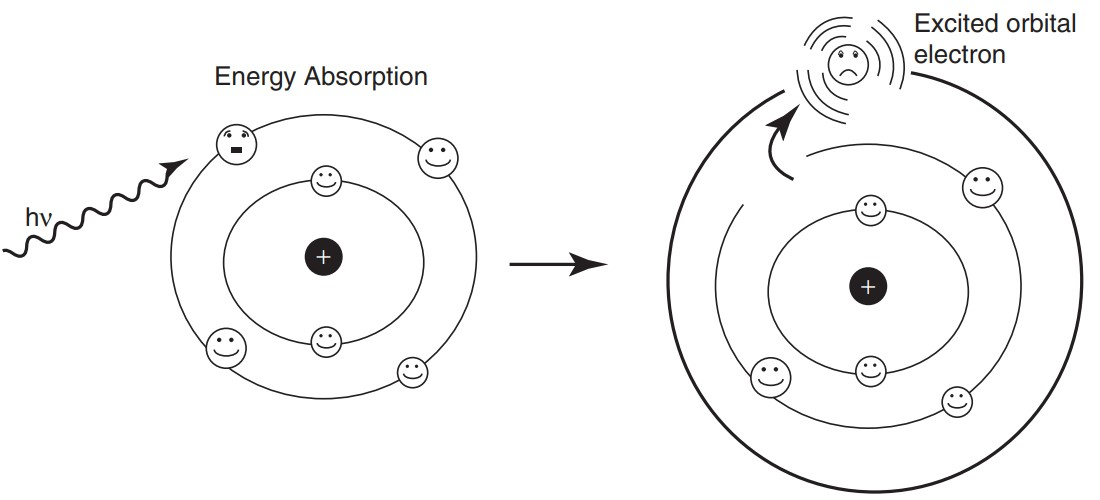
\includegraphics[width=0.7\textwidth]{Imagens/absorcaoDeEnergiaPorEletronOrbital.jpg}
                    \caption{Absorção de energia por um elétron orbital}
                    \label{fig:absorcaoDeEnergiaPorEletronOrbital}
                \end{figure}

                Sempre que um elétron é arrancado de uma das camadas mais internas do átomo, um elétron de uma camada mais externa, com maior energia, irá preencher esta vacância da camada mais interna, menos energética. Neste processo, haverá um excesso de energia que poderá ser emitido em forma de fótons, chamados de raios-x característicos ou pode ser transferida para um elétron orbital chamado elétron Auger, Figura \ref{fig:emissaoRaiosXCaracteristicosEEletronAuger}.

                \begin{figure}[h]
                    \centering
                    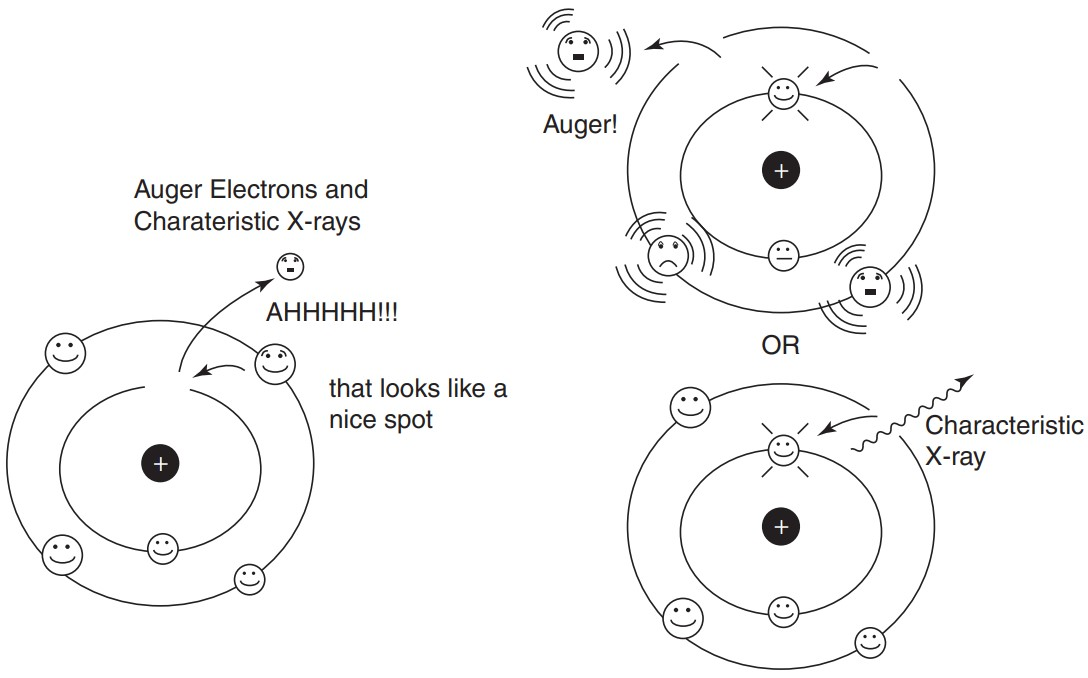
\includegraphics[width=0.7\textwidth]{Imagens/emissaoRaiosXCaracteristicosEEletronAuger.jpg}
                    \caption{Absorção de energia por um elétron orbital}
                    \label{fig:emissaoRaiosXCaracteristicosEEletronAuger}
                \end{figure}

                Os Raios-X característicos recebem este nome pois os níveis de energia de cada órbita são específicos para cada tipo de material e a energia do fóton emitido é igual a diferença de energia entre as camadas envolvidas na transição, que será única para cada tipo de elemento.
                
                Os elétrons Auger, saem com energia cinética igual a diferença de energia entre as camadas envolvidas na transição menos a energia de ligação deste elétron em sua respectiva órbita.


                O número de raios-x característicos emitidos por vacância é referido como produção fluorescente $w$, enquanto que o número de elétrons Auger emitidos por vacância é (1 - $w$). A produção fluorescente depende do número atômico Z do átomo e do número quântico principal da camada. Para átomos com Z $<$ 10, a produção fluorescente da camada k $W_k = 0$; Para Z de aproximadamente 30, $W_k \approx 0.5$ e para altos números atômicos, $w_k = 0.96$.


    \section{Radioatividade}

        A radioatividade é caracterizada como a transformação de elementos instáveis em busca da estabilidade. Este processo resulta, além da transformação nuclear, em emissão de energia e produtos de decaimento.
        
        
        \subsection{Modos de Decaimento Radioativo}

            Um processo de decaimento há sempre a conservação de carga massa e energia e pode ser descrito através de um esquema de reação, como exemplo abaixo:

            \begin{center}
                $\ce{^{226}_{88}Ra ->[{T_{1/2}}][{1,622y}] ^{222}_{86}Rn + ^{4}_{2}He + 4.87 MeV}$
            \end{center}

            A energia liberada no processo é compartilhada com os produtos do decaimento, que podem assumir espectros discretos, onde saem sempre com a mesma energia, ou com espectros contínuos, onde podem assumir qualquer energia dentro da energia máxima liberada no decaimento. Nos casos do espectro contínuo de energia, a energia média da partícula emitida pode ser obtida através da equação:
            
                \begin{equation}
                    \overline{E_k} = \frac{1}{3} E_{max}
                \end{equation}
            
            Os produtos produzidos nos processos de decaimento são:

            \begin{itemize}
                \item \textbf{\textit{\textcolor{CarnationPink}{Partícula $\alpha$}}}, um núcleo de Hélio;
                \item \textbf{\textit{\textcolor{CarnationPink}{Partícula $\beta^-$}}}, négatron, partícula semelhante ao elétron, diferindo apenas pela sua origen no núcleo;
                \item \textbf{\textit{\textcolor{CarnationPink}{Partícula $\beta^+$}}}, pósitron, antipartícula do elétron;
                \item \textbf{\textit{\textcolor{CarnationPink}{Raios $\gamma$}}}, fóton semelhante a radiação-x exceto por sua origem;
                \item \textbf{\textit{\textcolor{CarnationPink}{Elétron de conversão interna}}}, elétron ejetado de uma órbita devido ao excesso de energia no núcleo, que pode leva a emissão de raios-X característicos.
            \end{itemize}
        
            \subsubsection{Decaimento Alfa}

                É um modo de decaimento que ocorre com núcleos muito pesados, $Z > 52$, onde é emitido um núcleo de Hélio (partícula $\alpha$). O esquema abaixo mostra um processo de decaimento $\alpha$:

                \begin{center}
                    $\ce{^{226}_{88}Ra ->[{T_{1/2}}][{1,622y}] ^{222}_{86}Rn + ^{4}_{2}He + 4.87 MeV}$
                \end{center}

                A energia liberada nesse processo é quase totalmente convertida em energia cinética para a partícula $\alpha$, uma pequena quantidade é convertida em recuo do núcleo, portanto a partícula $\alpha$ possui um espectro discreto (monoenergético). 
            

            \subsubsection{Decaimento Beta-Menos}
                
                Ocorre em núcleos com excesso de nêutrons que precisam de mais prótons para se tornarem menos instáveis. O esquema abaixo é um exemplo de decaimento $\beta^-$:

                \begin{center}
                    $\ce{^{32}_{15}P ->[{T_{1/2}}][{14.5d}] ^{32}_{16}S + ^{0}_{-1}\beta \; + ^{0}_{0}\overline{\nu} \; + 1.7 MeV}$
                \end{center}

                Portanto, neste processo, um nêutron se transforma em um próton que é mantido no núcleo e ejeta uma partícula $\beta^-$ juntamente com um antineutrino.

                \begin{itemize}
                    \item A carga é conservada, $\ce{^{1}_{0} n -> ^{1}_{+1} p + ^{0}_{-1} e \; + ^{0}_{0} \overline{\nu}}$;
                    \item Como há a liberação de uma partícula, uma antipartícula também é liberada; 
                    \item A massa é conservada, e se trata de um decaimento isobárico, onde o número de massa atômica é conservado; pois perde-se um nêutron mas ganha-se um próton;
                    \item O número atômico é acrescido de 1 unidade; 
                    \item O espectro de energia da partícula $\beta^-$ é contínuo (polienergético) pois a energia liberada na reação é compartilhada entre a partícula beta e o antineutrino.
                \end{itemize}

            \subsubsection{Decaimento Beta-Mais}

                Ocorre em núcleos com excesso de prótons que precisa de mais nêutrons para se tornarem menos instáveis. O esquema abaixo demonstra um exemplo de decaimento $\beta^+$:

                \begin{center}
                    $\ce{^{18}_{9} F ->[{T_{1/2}}][{110 min}] ^{18}_{8} O + ^{0}_{+1} \beta \; + ^{0}_{0} \nu \; + 0.63 MeV}$
                \end{center}

                Neste processo, um próton é convertido em um nêutron que é absorvido pelo núcleo e é emitido um pósitron e um neutrino.

                \begin{itemize}
                    \item A carga é conservada, $\ce{^{1}_{1} p -> ^{0}_{0} n + ^{1}_{+1} e + ^{0}_{0} \nu}$;
                    \item Como há a liberação de uma antipartícula, uma partícula também é liberada;
                    \item A massa é conservada, e se trata de um decaimento isobárico, onde o número de massa atômica é conservado pois perde-se um próton mas ganha-se um nêutron;
                    \item O número atômico é diminuído em 1 unidade;
                    \item O espectro de energia da partícula $\beta^+$ é contínuo (polienergético) pois a energia liberada na reação é compartilhada entre a partícula beta e o neutrino;
                \end{itemize}

                Ao ser liberado no meio, esse pósitron irá diminuir sua energia até que, por ser uma antimatéria com massa, sofra uma interação com um elétron do meio resultando no processo chamado de aniquilação de pares. Nesse processo o pósitron e o elétron se aniquilam liberando sua energia de repouso em forma de fótons. A energia de repouso de um elétron é de \qty{0.511}{MeV} e portanto são liberados 2 fótons idênticos com energia de \qty{0.511}{MeV} em direções opostas. 

                É necessário então uma energia de \qty{1.022}{MeV} para criar um pósitron, portanto se a energia cinética no decaimento for menor que este valor, para conseguir um neutron, o núcleo decairá através da captura eletrônica.

            \subsubsection{Captura Eletrônica}

                Ocorre em núcleos com excesso de prótons mas que não são energéticos o suficiente para criar um pósitron. O esquema abaixo demonstra um exemplo de decaimento por captura eletrônica.

                \begin{center}
                    $\ce{^{125}_{53} I +  ^{0}_{-1} e \; ->[{T_{1/2}}][{59.4 d}] \; ^{125}_{52} Te +  ^{0}_{0} \nu \; + 35.5 MeV}$
                \end{center}

                Neste processo, um elétron orbital é capturado que juntamente com um  próton do núcleo e com ação da força fraca formam um neutron e na sequência é emitido um neutrino.

                Como os demais processos, a carga é conservada. O número atômico para a CE é decrescido de 1 unidade mas a massa atômica se mantém a mesma. Embora seja emitido um neutrino, a maior parte da energia liberada no decaimento por captura eletrônica é mantida no núcleo filho, que posteriormente será emitida através de radiação gama ou por um processo de conversão interna.

                \textbf{\textit{\textcolor{CarnationPink}{Obs:}}} Nucleos ricos em prótons com energia insuficiente para criar um pósitron decaem apenas por captura eletrônica, já os núcleos muito energéticos ricos em prótons podem decair ou por emissão de pósitron ou por captura eletrônica.

                Como uma vacância em uma camada interna do átomo é formada, consequentemente ocorrerá a emissão de um raio-x característico ou de um elétron Auger; E caso o excesso de energia seja liberado através da conversão interna, outra vacância será formada. A Figura \ref{fig:decaimentoPorCapturaEletronica} exemplifica o processo de captura eletrônica que resulta em um núcleo filho que decai por $\beta^+$.

                \begin{figure}[h]
                    \centering
                    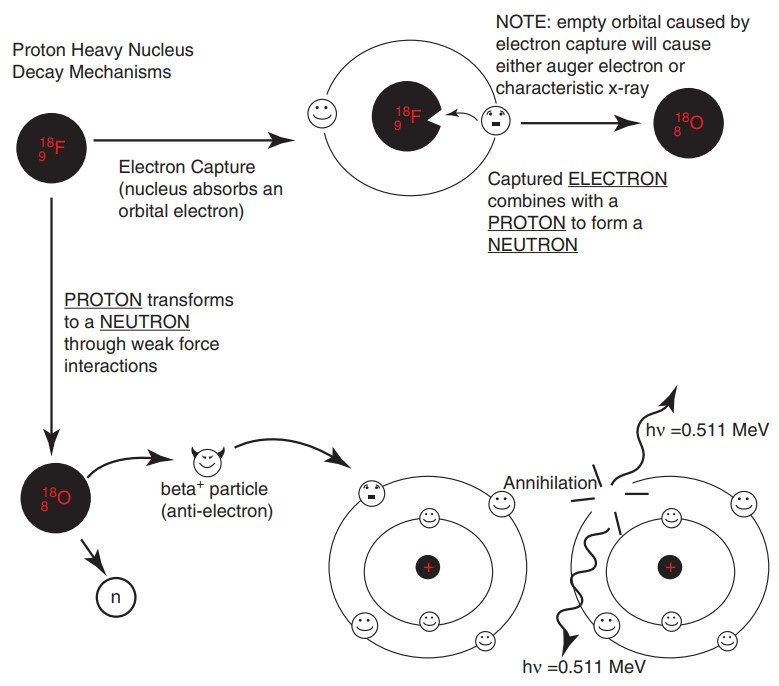
\includegraphics[width=0.7\textwidth]{Imagens/decaimentoPorCapturaEletronica.jpg}
                    \caption{Decaimento por captura eletrônica}
                    \label{fig:decaimentoPorCapturaEletronica}
                \end{figure}

            \subsubsection{Emissão Gama}

                Após o decaimento, o núcleo filho pode permanecer com um excesso de energia, chamado de estado excitado, sendo necessário liberar este excesso de energia e uma das formas é emitindo um fóton. Um exemplo de emissão gama é demonstrado abaixo:

                \begin{center}
                    $\ce{^{60}_{27} Co  ->[{T_{1/2}}][{5.26 y}] \; ^{60}_{28} Ni + ^{0}_{-1}\beta \; + ^{0}_{0}\overline{\nu} \; + 0.31 MeV + 1.17 MeV (\gamma) + 1.33 MeV (\gamma)}$
                \end{center}
                
                A emissão gama é sempre isomérica, e para o exemplo citado, a radiação gama é imediatamente emitida. Em alguns casos, é possível que o núcleo filho possa brevemente existir em um estado excitado, chamado de Núcleos Metaestáveis, antes de liberar sua energia, como ocorre com o \ce{^{99m}_{43}Tc}.

                \begin{center}
                    $\ce{^{99m}_{43} Tc ->[{T_{1/2}}][6.0 h] ^{99}_{43} Tc + 140.5 KeV}$
                \end{center}
            
            \subsubsection{Conversão Interna}

                
                Ocorre quando um núcleo, ao invés de liberar sua energia emitindo um fóton, transfere esse excesso de energia para um dos elétrons orbitais pertencente às camadas mais internas do átomo.  Esse elétron irá sair com a energia cinética igual a diferença entre a energia transferida para o elétron e a energia de ligação do elétron, que irá depender de qual camada este elétron pertence. Uma vez que diferentes elétrons possuem diferentes energias de ligação, a conversão interna resultará em um espectro de energias. A Figura \ref{fig:processoDeConversaoInterna} mostra a sequência de eventos que ocorrem durante a conversão interna.


                \begin{figure}[h]
                    \centering
                    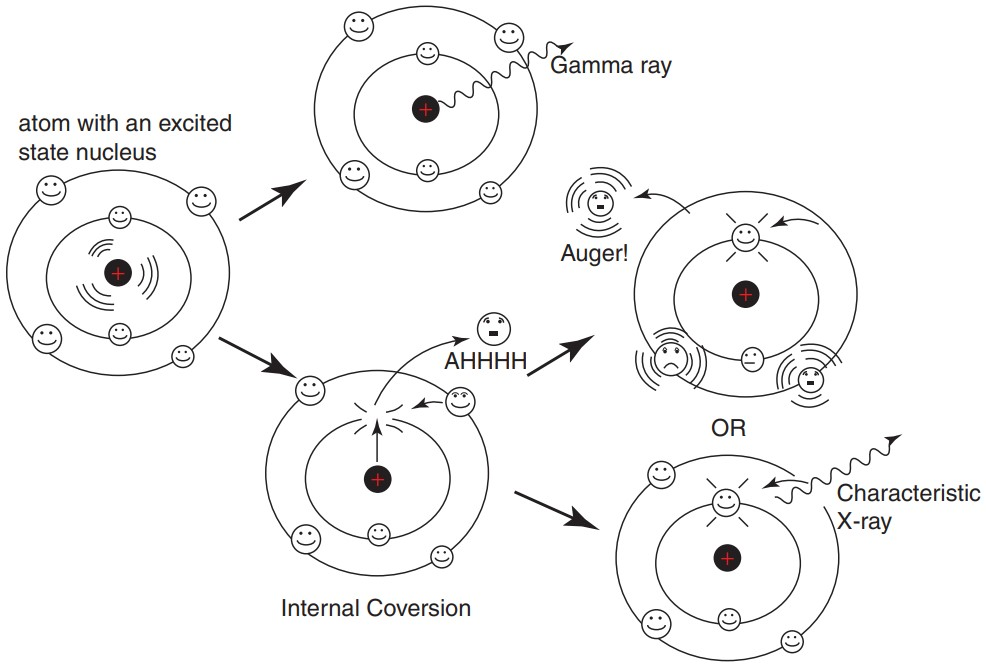
\includegraphics[width=0.7\textwidth]{Imagens/processoDeConversaoInterna.jpg}
                    \caption{Conversão Interna}
                    \label{fig:processoDeConversaoInterna}
                \end{figure}


        \subsection{Lei de Decaimento Exponencial}

            A lei de decaimento exponencial é quem governa o decaimento e crescimento de substâncias radioativas e através dela é possível obter parâmetros que caracterizam uma amostra de substância radioativa.
            
            \begin{itemize}
                \item A Atividade de uma substância radioativa em um tempo $t$, $\mathcal{A}(t)$ é definida como o produto da constante de decaimento $\lambda$ pelo número de átomos radioativos no tempo $t$, $N(t)$ é dada pela equação:

                    \begin{equation}
                        \mathcal{A} (t) = \lambda N(t)
                    \end{equation}

                \item O número de núcleos pai radioativos $N_p$ em função do tempo $t$ é dado pela equação:
                    
                    \begin{equation}
                        N_p(t) = N_{p_0} \; e^{-\lambda_P t}
                    \end{equation}

                    onde $N_{p_0}$ é o número inicial de átomos radioativos, ou seja, número de átomos radioativos em t = 0.

                \item A Atividade do núcleo pai $\mathcal{A}_p$ em função do tempo $t$ é obtida através da equação:
                
                    \begin{equation}
                        \mathcal{A}_p(t) = \mathcal{A}_{p_0} \; e^{-\lambda_P t}
                    \end{equation}
                    
                    onde $\mathcal{A}_{p_0}$ é a atividade inicial do núcleo pai, ou seja, atividade em t = 0;

                \item A meia-vida de uma substância radioativa $(t_{1/2})$ é definida como a duração de tempo necessária para que o número de núcleos radioativos decaia para metade do seu valor inicial, ou seja, para que o número de núcleos radioativos seja a metade do valor presente em t = 0:
                
                    \begin{equation}
                        N_p(t = t_{1/2}) = \frac{1}{2} N_{p_0} = N_{p_0} \; e^{-\lambda_P t_{1/2}}
                    \end{equation}
                
                \item A meia-vida $(t_{1/2})$ e a constante de decaimento $\lambda_P$ podem ser relacionadas através da seguinte equação:
                
                    \begin{equation}
                        \lambda_P = \frac{\ln 2}{t_{1/2}}
                    \end{equation}

                \item A atividade específica $a$ é definida como a atividade do núcleo pai por unidade de massa:
                
                    \begin{equation}
                        a = \frac{\mathcal{A}_p}{m} = \frac{\lambda_P \; N}{m} = 
                        \lambda_P \frac{N_A}{\mathbb{A}_p} = \frac{N_A \; \ln 2}{\mathbb{A}_p (t_{1/2})_p}
                    \end{equation}
                
                    onde $N_A$ é a constante de Avogadro e $\mathbb{A}_p$ é o número de massa atômica do núcleo pai.
                
                \item A vida média $\tau_p$ de uma substância radioativa representa a expectativa de vida média de todos os átomos pais radioativos na substância a partir do tempo t = 0. É uma quantidade de tempo hipotética que uma fonte levaria para decair completamente se a fonte decaísse com uma taxa constante igual a atividade inicial.
                
                    \begin{equation}
                        \mathcal{A}_{p_0} \; \tau_p = 
                        \int_{0}^{\infty} \mathcal{A}_{p_0} e^{-\lambda_P \; t} \,dt = 
                        \frac{\mathcal{A}_{p_0}}{\lambda_P}
                    \end{equation}

                e portanto, a vida-média está relacionada com a constante de decaimento e com a meia vida através da equação:

                    \begin{equation}
                        \tau_p = \frac{1}{\lambda_P} = \frac{t_{1/2}}{\ln 2} = 1.44 \; t_{1/2}
                    \end{equation}
            \end{itemize}

            \subsubsection{Equilibrio Radioativo}

                Quando ocorrem sucessivos decaimentos radioativos, cada novo elemento terá seu próprio tempo de meia-vida e portanto no decorrer do tempo poderá ser alcançado um equilíbrio; Quando um núcleo pai P decai, com uma constante de decaimento $\lambda_P$ para um núcleo filho D que também decai, com uma constante de decaimento $\lambda_D$ para um núcleo estável G temos que: 
                
                \noindent A atividade do núcleo filho pode ser determinada através da expressão:

                \begin{equation}
                    \mathcal{A}_D(t) = \frac{\lambda_D}{\lambda_D - \lambda_P} \mathcal{A}_{p_0}\left(e^{-\lambda_P t} - e^{-\lambda_D t}\right)
                \end{equation}


                \noindent A atividade máxima do núcleo filho ocorre em $t_{max}$ dado por:

                \begin{equation}
                    t_{max} = \frac{\ln (\lambda_D / \lambda_P)}{\lambda_D - \lambda_P}
                \end{equation}

                \begin{itemize}
                    \item \textbf{\textit{\textcolor{CarnationPink}{Ausência de Equilíbrio}}}
                \end{itemize}

                    Ocorre quando a meia-vida do núcleo filho é maior que a meia-vida do núcleo pai e portanto todo núcleo pai decai para o núcleo filho não sendo possível chegar em um ponto que as atividades entrem em equilíbrio.

                    Portanto, para $\lambda_D < \lambda_P$, o que é o mesmo que  $(t_{1/2})_D > (t_{1/2})_P $ a relação entre a atividade do núcleo filho com a atividade do núcleo pai é dada por:

                        \begin{equation}
                            \frac{\mathcal{A}_D}{\mathcal{A}_P} = 
                            \frac{\lambda_D}{\lambda_D - \lambda_P} \left[1 - e^{-(\lambda_D - \lambda_P)t}\right]
                        \end{equation}
                
                    Um exemplo de ausência de equilíbrio está no decaimento do Telúrio-131 para o Iodo-131, onde a meia-vida do \ce{^{131}_{52}Te} é de 30h e a meia-vida do \ce{^{131}_{52}I} é de 192h.

                \begin{itemize}
                    \item \textbf{\textit{\textcolor{CarnationPink}{Equilíbrio Secular}}}
                \end{itemize}
        
                    Ocorre quando a meia-vida do núcleo filho é muito menor que a meia-vida do núcleo pai. Neste caso o núcleo filho é produzido na velocidade com o qual o núcleo pai decai e portanto a atividade do núcleo filho tem um período de buildup de forma que ela aumenta gradativamente até que a atividade do núcleo filho fique aproximadamente igual a atividade do núcleo pai. 

                    \begin{equation}
                        \frac{\mathcal{A}_D}{\mathcal{A}_P} \approx 1
                    \end{equation}

                    \begin{figure}[h]
                        \centering
                        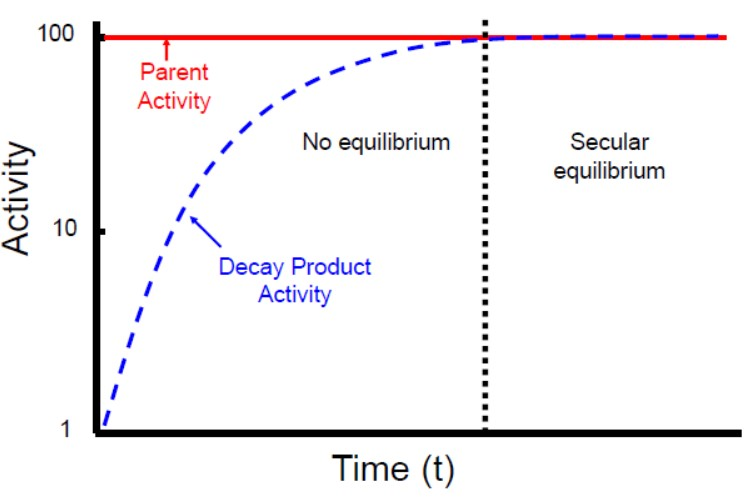
\includegraphics[width=0.7\textwidth]{Imagens/graficoEquilibrioSecular.jpg}
                        \caption{Equilíbrio Secular}
                        \label{fig:graficoEquilibrioSecular}
                    \end{figure}

                    O equilíbrio secular ocorre no decaimento do Rádio-226 para o Radônio-222 onde a meia-vida do \ce{^{226}_{88}Ra} é de 1620 anos e a meia vida do \ce{^{222}_{86}Rn} é de 4.8 dias. Outro exemplo é o decaimento do Estrôncio-90 para o Ítrio-90, onde o \ce{^{90}_{38}Sr} possui meia-vida de 29.12 anos e o \ce{^{90}_{39}Y} tem meia-vida de 64h.

                \begin{itemize}
                    \item \textbf{\textit{\textcolor{CarnationPink}{Equilíbrio Transiente}}}
                \end{itemize}

                    Ocorre quando o núcleo filho possui meia-vida ligeiramente menor que a meia-vida do núcleo pai. A atividade do filho começa a crescer a medida que o pai decai. Em um determinado momento, a atividade do filho excede ligeiramente a atividade do pai e ambas atividades começam a diminuir juntas. Neste caso a  a atividade do núcleo filho parece ser maior que a do núcleo pai e ambos parecem ter a mesma meia-vida.
                    
                    \begin{equation}
                        \frac{\mathcal{A}_D}{\mathcal{A}_P} = \frac{\lambda_D}{\lambda_D - \lambda_P} \qquad para \quad t \gg t_{max}
                    \end{equation}
                
                    \begin{figure}[h]
                        \centering
                        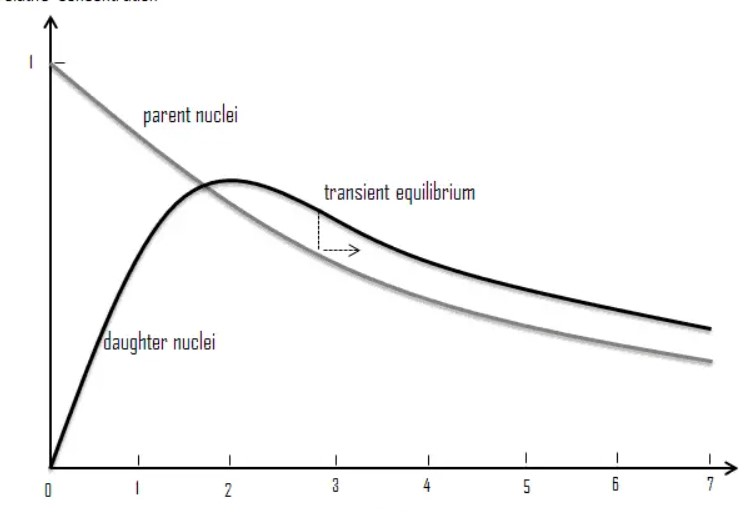
\includegraphics[width=0.7\textwidth]{Imagens/graficoEquilibrioTransiente.jpg}
                        \caption{Equilíbrio Transiente}
                        \label{fig:graficoEquilibrioTransiente}
                    \end{figure}

                    Um exemplo de equilíbrio transiente ocorre no decaimento do Molibdênio-99 para o Tecnécio-99 metaestável, onde o \ce{^{99}_{42}Mo} possui meia-vida de 66h e o \ce{^{99m}_{43}Tc} possui meia-vida de 6h.
                
            \subsubsection{Eluição do Núcleo Filho}

                Utiliza um gerador do radionuclídeo para extrair o núcleo filho gerado pelo núcleo pai. A cada vez que o núcleo filho é removido, ocorre um novo período de buildup até que seja alcançado novamente o equilíbrio secular ou transiente. Um exemplo é o gerador de \ce{^{99m}_{43}Tc},Figura \ref{fig:graficoEluicaoTecnecio}.


                    \begin{figure}[h]
                        \centering
                        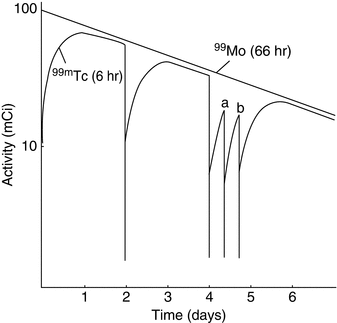
\includegraphics[width=0.5\textwidth]{Imagens/graficoEluicaoTecnecio.jpg}
                        \caption{Eluição do Tecnécio-99m}
                        \label{fig:graficoEluicaoTecnecio}
                    \end{figure}

                Um gerador de \ce{^{99m}_{43}Tc} utiliza como o núcleo pai o \ce{^{99}_{42}Mo} que é fixado em uma coluna alumina ou de outro material poroso. Sempre que o \ce{^{99}Mo} decai, é gerado um núcleo de \ce{^{99m}Tc} que fica retido na coluna. Para remover o \ce{^{99m}Tc} utiliza-se um eluente, que normalmente é uma solução de cloreto de sódio, que dissolve o \ce{^{99m}Tc} retido na coluna e então o \ce{^{99m}Tc} eluído é removido do gerador. A eficiência na produção de \ce{^{99m}Tc} a partir do \ce{^{99}Mo} é de aproximadamente 88\%.
             
        \subsection{Elementos Radioativos}
            
            Os elementos radioativos podem ser encontrados naturalmente ou podem ser produzidos artificialmente envolvendo processos que levam à transformação do núcleo.

            \subsubsection{Séries Radiotivas}
            
                Alguns elementos radioativos encontrados naturalmente pertencem a séries de decaimento bem definidas. Essas séries são classificadas como:
                
                

                \begin{itemize}
                    \item \textbf{\textit{\textcolor{CarnationPink}{Série do Tório (4n):}}} Esta série começa com o Tório-232 (\ce{^{232}Th}) e termina com o isótopo estável Chumbo-208 (\ce{^{208}Pb}), Figura \ref{fig:serieDoTorio}.

                    \begin{figure}[h]
                        \centering
                        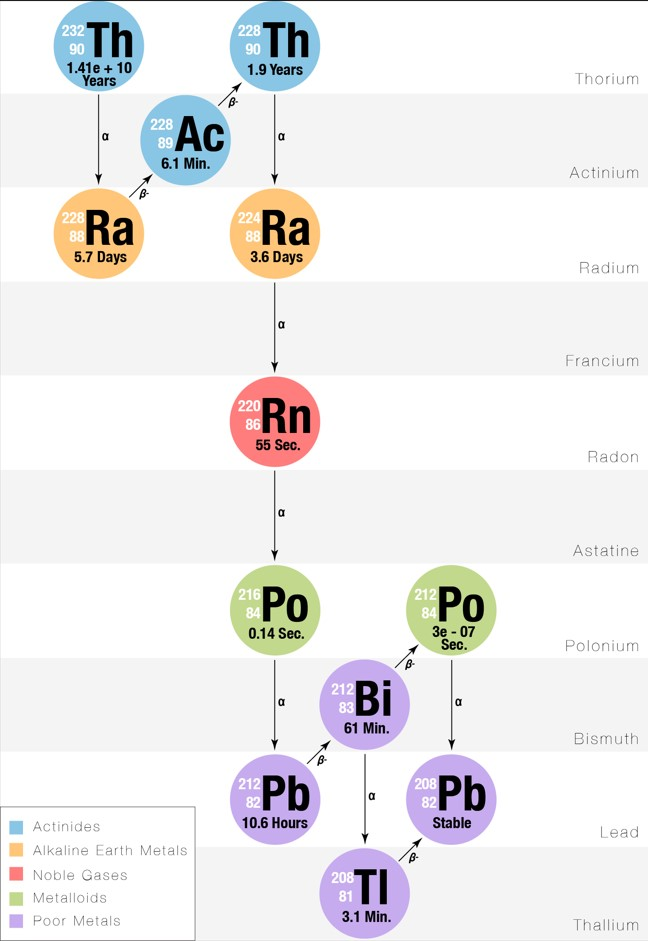
\includegraphics[width=0.4\textwidth]{Imagens/serieDoTorio.jpg}
                        \caption{Série do Tório-232}
                        \label{fig:serieDoTorio}
                    \end{figure}

                    Essa série é chamada de 4n porque muitos dos isótopos intermediários têm um número de massa igual a quatro vezes um número inteiro (4n), onde n é um número inteiro.

                        \textbf{Exemplo}: \textit{o primeiro isótopo intermediário na série é o rádio-228 (\ce{^{228}Ra}) , que tem um número de massa de 228. O número 228 é igual a 4 vezes 57, o que corresponde a n = 57 na equação 4n. O segundo isótopo intermediário na série é o actínio-228 (\ce{^{228}Ac}), que também tem um número de massa de 228. Novamente, o número 228 é igual a 4 vezes 57.}

                        Esse padrão de diferença de número de massa de 4n é observado em muitos dos isótopos intermediários da série do tório, como resultado do processo de decaimento radioativo. A série do tório é importante na geologia, pois a taxa de decaimento dos isótopos intermediários é usada para determinar a idade de rochas e minerais, por meio de técnicas como a datação por tório-urânio. Além disso, alguns isótopos intermediários da série do tório, como o protactínio-234 (\ce{^{234}Pa}) e o rádio-223 (\ce{^{223}Ra}), são utilizados em aplicações médicas e industriais.

                    \item \textbf{\textit{\textcolor{CarnationPink}{Série do Neptúnio (4n + 1):}}}: Esta série começa com o Neptúnio-237 (\ce{^{237}Np}) e termina com o isótopo estável Bismuto-209 (\ce{^{209}Bi}), Figura \ref{fig:serieDoNeptunio}. 
                    
                        \begin{figure}[h]
                            \centering
                            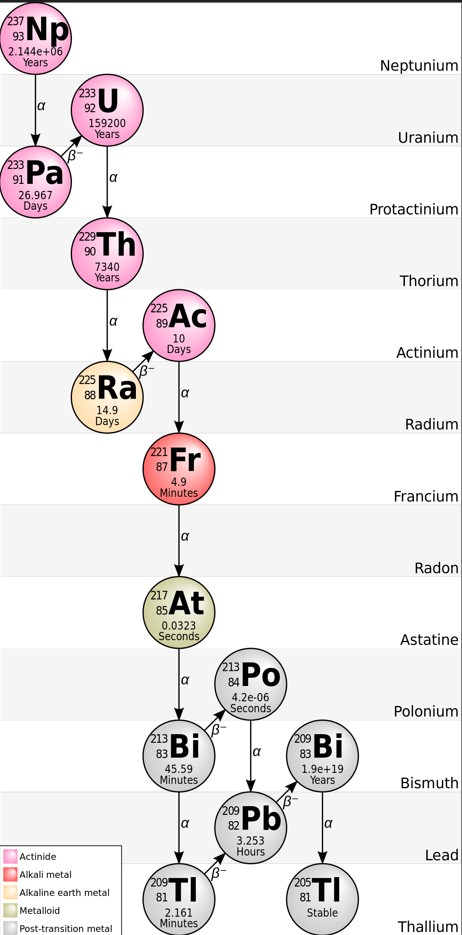
\includegraphics[width=0.4\textwidth]{Imagens/serieDoNeptunio.jpg}
                            \caption{Série do Neptúnio-237}
                            \label{fig:serieDoNeptunio}
                        \end{figure}
                    
                        Essa série é chamada de 4n + 1 porque muitos dos isótopos intermediários têm um número de massa igual a quatro vezes um número inteiro mais um (4n + 1), onde n é um número inteiro.
                    
                        \textbf{Exemplo}: \textit{ o primeiro isótopo intermediário na série é o protactínio-233 (233Pa), que tem um número de massa de 233. O número 233 é igual a 4 vezes 58 mais 1, o que corresponde a n = 58 na equação 4n + 1. O segundo isótopo intermediário na série é o urânio-233 (233U), que também tem um número de massa de 233. Novamente, o número 233 é igual a 4 vezes 58 mais 1.}

                        Esse padrão de diferença de número de massa de 4n + 1 é observado em muitos dos isótopos intermediários da série do neptúnio, como resultado do processo de decaimento radioativo. A série do neptúnio é menos conhecida e menos estudada do que as séries do urânio e do tório, devido à escassez de fontes naturais de neptúnio e à sua elevada radioatividade, mas ainda tem importância na ciência nuclear e em algumas aplicações industriais.

                    \item \textbf{\textit{\textcolor{CarnationPink}{Série do Urânio (4n + 2):}}} Esta série começa com o Urânio-238 (\ce{^{238}U}) e termina com o isótopo estável Chumbo-206 (\ce{^{206}Pb}), Figura \ref{fig:serieDoUranio}. 
                    
                            \begin{figure}[h]
                                \centering
                                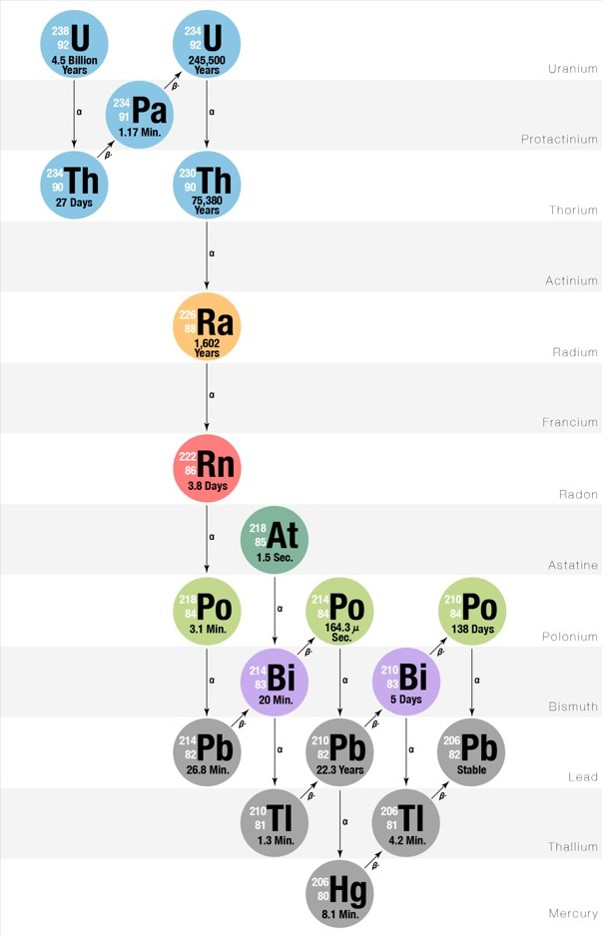
\includegraphics[width=0.4\textwidth]{Imagens/serieDoUranio.jpg}
                                \caption{Série do Urânio-238}
                                \label{fig:serieDoUranio}
                            \end{figure}
                    
                        
                        Essa série é chamada de "4n + 2" porque muitos dos isótopos intermediários têm um número de massa igual a quatro vezes um número inteiro mais dois (4n + 2), onde n é um número inteiro.

                        \textbf{Exemplo}: \textit{o primeiro isótopo intermediário na série é o tório-234 (\ce{^{234}Th}), que tem um número de massa de 234. O número 234 é igual a 4 vezes 58 mais 2, o que corresponde a n = 58 na equação 4n + 2. O segundo isótopo intermediário na série é o protactínio-234 (\ce{^{234}Pa}), que também tem um número de massa de 234. Novamente, o número 234 é igual a 4 vezes 58 mais 2.}
                    
                        Esse padrão de diferença de número de massa de 4n + 2 é observado em muitos dos isótopos intermediários da série do urânio, como resultado do processo de decaimento radioativo. A série do urânio-238 é importante porque o urânio-238 é um elemento relativamente comum na crosta terrestre e é usado como combustível em reatores nucleares e como material para a produção de armas nucleares.


                    \item \textbf{\textit{\textcolor{CarnationPink}{Série do Actínio (4n + 3):}}} Esta série começa com o Urânio-235 (\ce{^{235}U}) e termina com o isótopo estável Chumbo-207 (\ce{^{207}Pb}), Figura \ref{fig:serieDoActinio}. 
                    
                    
                        \begin{figure}[h]
                            \centering
                            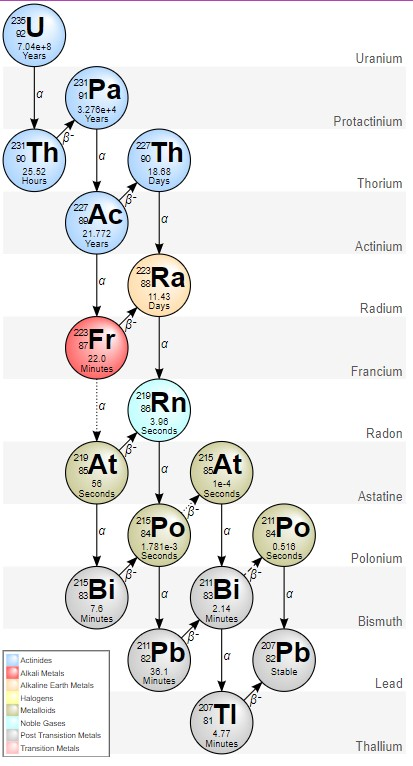
\includegraphics[width=0.4\textwidth]{Imagens/serieDoActinio.jpg}
                            \caption{Série do Actínio: Urânio-235}
                            \label{fig:serieDoActinio}
                        \end{figure}
                    
                        Essa série é chamada de "4n + 3" porque muitos dos isótopos intermediários têm um número de massa igual a quatro vezes um número inteiro mais dois (4n + 3), onde n é um número inteiro.

                        \textbf{Exemplo}: \textit{o primeiro isótopo intermediário na série é o tório-231 (234Th), que tem um número de massa de 231. O número 231 é igual a 4 vezes 57 mais 3, o que corresponde a n = 57 na equação 4n + 3. O segundo isótopo intermediário na série é o protactínio-231 (234Pa), que também tem um número de massa de 231. Novamente, o número 231 é igual a 4 vezes 57 mais 3.}

                        Vários isótopos intermediários da série do actínio, como o rádio-223, têm aplicações em medicina, como no tratamento de certos tipos de câncer (Xofigo). A série do actínio também é importante na pesquisa nuclear e no estudo da geologia. lém disso, alguns isótopos como o urânio-235 (\ce{^{235}U}) e o plutônio-239 (\ce{^{239}Pu}), são utilizados em aplicações industriais e militares.

                \end{itemize}
                
                Alguns elementos radioativos encontrados naturalmente não pertencem a alguma série radiativa, sendo eles: Hidrogênio-3 (\ce{^{3}H} - tritium),  Carbono-14 (\ce{^{14}C}), Potássio-40 (\ce{^{40}K}), Vanádio-50 (\ce{^{50}V}), Rubídio-87 (\ce{^{87}Rb}), Índio-115 (\ce{^{115}In}), Telúrio-130 (\ce{^{130}Te}), Lantânio-138 (\ce{^{138}La}), Cério-142 (\ce{^{142}Ce}), Neodímio-144 (\ce{^{144}Nd}), Samário-147 (\ce{^{147}Sm}), Lutécio-176 (\ce{^{176}Lu}), Rênio-187 (\ce{^{187}Re}) e Platina-192 (\ce{^{192}Pt}).
            
            \subsubsection{Radiatividade Artificial}

                Alguns elementos radioativos não são encontrados naturalmente, pois são produzidos artificialmente através do bombardeamento nuclear com partículas. Em um bombardeamento nuclear, um núcleo estável é bombardeado com prótons, neutrons ou outras partículas para gerar núcleos radiativos.

                No bombardeamento com prótons, frequentemente são criados emissores de pósitrons como o \ce{^{18}F} utilizada em PET scans, mas também podem causar outras reações:

                    \begin{itemize}
                        \item $(p, \gamma)$: um próton é incorporado pelo núcleo, excitando-o e essa energia é liberada em forma de radiação gama.
                        \item $(p, n)$: o próton é incorporado pelo núcleo que libera um neutron;
                        \item $(p, d)$: o próton é incorporado pelo núcleo que libera um deutério;
                    \end{itemize}

                Outras partículas carregadas pesadas, como partícula alfa, e deutérios \ce{^{2}H}, também podem ser utilizados no bombardeamento. Ambas são capazes de ser incorporadas pelo núcleo que resulta na  liberação de prótons ou neutrons.

                Em um bombardeamento com neutrons, quanto mais próximo o neutron fica do núcleo, maior a probabilidade de ocorrer uma reação nuclear. Para isto os neutrons precisam estar com energia cinética de aproximadamente \qty{0.025}{eV}, os chamados neutrons térmicos. As possíveis reações que podem ocorrer devido a incorporação do neutron pelo núcleo são:

                \begin{itemize}
                    \item \ce{(n, \gamma)}: O núcleo captura o neutron e fica em um estado excitado, liberando este excesso de energia em forma de radiação gama. Exemplo: \ce{^{1}H + n -> ^{2}H + \gamma}
                    
                    \item \ce{(n, \alpha)}: O núcleo absorve o neutron e emite uma partícula alfa no processo de desexcitação. Exemplo: \ce{^{10}B + n -> ^{7}Li + ^{4}He}, esta é a reação base para detecção de neutrons.
                    
                    \item \ce{(n, p)}: o núcleo absorve o neutron e emite um próton. Exemplo: \ce{^{32}S + n -> ^{32}P + ^{1}H+}
                    
                    \item \textbf{Fissão Nuclear:} Quando o \ce{^{235}U} ou \ce{^{239}Pu} (Plutônio) são bombardeados com neutrons, ao absorverem neutrons térmicos, os núcleos se quebram em dois produtos principais com massas diferentes, em torno de 90 - 100 e 130 - 140 juntamente com neutrons ou outros núcleos menores e grande quantidade de energia. Muitas fontes mostram que o \ce{^{235}U} se quebra em \ce{^{92}Kr} (Criptônio) e \ce{^{114}Ba} (Bário) com 3 neutrons e libera uma energia de \qty{200}{MeV}.
                    
                        O \ce{^{238}U} consiste em 99.2\% de todo Urânio natural e é menos propenso a sofrer uma fissão e  sustentar uma reação em cadeia. Para aumentar a proporção do \ce{^{235}U} é realizado um procedimento chamado de Enriquecimento de Urânio de forma que aumente a habilidade de sustentar uma fissão nuclear. Urânio pouco enriquecido (3\% - 4\% de \ce{^{235}U}) é utilizado em Usinas de Energia embora algumas utilizem o Urânio não-enriquecido. Para armas nucleares é necessário um mínimo de 20\% de \ce{^{235}U} e países desenvolvidos utilizam Urânio enriquecido com 80\% - 90\% de \ce{^{235}U} ou o \ce{^{239}Pu}.

                        No processo de fissão, os neutrons liberados causam outras fissões e uma reação em cadeia pode ser sustentada quando se atinge uma massa crítica. Em usinas nucleares de energia, uma reação em cadeia é controlada através da absorção dos neutrons utilizando boro, cádmio (Cd) ou água. Já em Armas Nucleares, o objetivo é não controlar a reação em cadeia! 
                \end{itemize}

            \subsubsection{Enriquecimento De Urânio}

                O enriquecimento de urânio é o processo pelo qual o urânio é transformado em urânio enriquecido, que é usado como combustível em reatores nucleares. Existem diferentes métodos para enriquecer urânio, mas o mais comum é o processo de centrifugação.

                O processo começa com a mineração de urânio, que envolve a extração do minério de urânio da crosta terrestre. O minério de urânio é então convertido em um gás chamado hexafluoreto de urânio (\ce{UF6}), que é o material de alimentação para o processo de enriquecimento.
                
                No processo de centrifugação, o \ce{UF6} é colocado em uma centrífuga, que é uma máquina que gira a uma velocidade muito alta. O centrifugado é o material enriquecido, enquanto o resíduo é o material empobrecido. O processo é repetido várias vezes em uma cascata de centrifugas, produzindo urânio enriquecido de maior grau a cada estágio.
                
                Outro método para enriquecer urânio é o processo de difusão gasosa, que envolve a passagem de \ce{UF6} através de uma membrana porosa. As moléculas mais leves de \ce{^{235}U} passam mais facilmente pela membrana do que as moléculas mais pesadas de \ce{^{238}U}, resultando em urânio enriquecido.

            \subsubsection{Reatores Nucleares}

                Um reator nuclear é um dispositivo que usa urânio enriquecido como combustível para produzir calor, que é usado para gerar eletricidade ou para outras finalidades. Existem vários tipos de reatores nucleares, mas o mais comum é o reator de água pressurizada (PWR, na sigla em inglês).

                No reator PWR, esquematicamente demonstrado na Figura \ref{fig:reatorNuclear}, o combustível nuclear é colocado em varetas de combustível e inserido em um núcleo do reator, que é preenchido com água. O urânio enriquecido dentro das varetas de combustível sofre fissão nuclear, liberando energia na forma de calor. O calor é transferido para a água do reator, que é mantida sob alta pressão para evitar que ferva.
                

                    \begin{figure}[h]
                        \centering
                        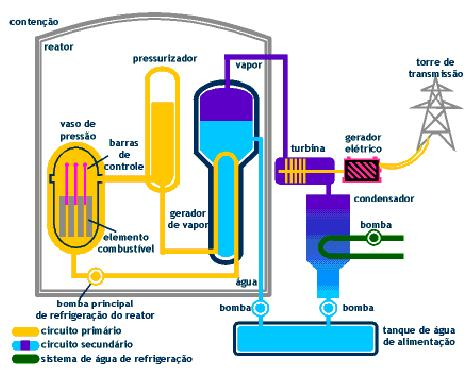
\includegraphics[width=0.5\textwidth]{Imagens/reatorNuclear.jpg}
                        \caption{Reator Nuclear de Água Pressurizada.}
                        \label{fig:reatorNuclear}
                    \end{figure}

                A água pressurizada é então bombeada para um trocador de calor, onde o calor é transferido para outro circuito de água que está a uma pressão mais baixa. A água do circuito secundário é convertida em vapor, que é usado para girar as pás de uma turbina, gerando eletricidade. Depois de passar pela turbina, o vapor é resfriado em um condensador e volta a ser água, que é bombeada de volta para o trocador de calor.
                
                O reator nuclear é controlado através da inserção e retirada de hastes de controle de nêutrons, que são feitas de materiais que absorvem nêutrons como o boro, na forma de ácido bórico ou na forma de metal e o cádmio em barras metálicas. Ao retirar as hastes, mais nêutrons são permitidos a atingir o combustível, aumentando a taxa de fissão e produzindo mais calor. Ao inserir as hastes, a taxa de fissão é reduzida, controlando a quantidade de calor produzida.

                Nos Reatores Nucleares do tipo PWR, é necessário haver a proporção de 32 átomos de \ce{^{235}U} para 968 átomos de \ce{^{238}U}, em cada grupo de 1.000 átomos de urânio, ou seja, 3,2\% de \ce{^{235}U}. Se o grau de enriquecimento for muito alto (acima de 90\%), isto é, se houver quase só urânio-235, pode ocorrer uma reação em cadeia muito rápida, de difícil controle, mesmo para uma quantidade relativamente pequena de urânio, passando a constituir-se em uma explosão, o que é buscado na bomba atômica.
                
                Os reatores nucleares são projetados com muitos sistemas de segurança para garantir que o combustível nuclear seja mantido sob controle e que o calor produzido seja gerenciado de forma segura. Por exemplo, se a temperatura ou pressão da água no reator ultrapassar níveis seguros, os sistemas de segurança são projetados para interromper a reação em cadeia e desligar o reator.
                
                \

                \noindent \textbf{\textit{\textcolor{CarnationPink}{Obs:}}} As principais fontes utilizadas em Radioterapia, como o \textbf{\ce{^{90}Sr}, \ce{^{90}Y}, \ce{^{131}I}, \ce{^{89}Sr}, \ce{^{192}I}, \ce{^{60}Co}} e o \textbf{\ce{^{137}Cs}} são produzidos em reatores nucleares.  
    
    \section{Produção e Propriedades da Radiação}
        
        \subsection{Classificação da Radiação}

            A radiação pode ser classificada quanto a sua natureza, partícula ou onda eletromagnética, e quanto ao seu poder de ionização, não-ionizante, diretamente ionizante e indiretamente-ionizante.

            As radiações particulada são definidas como as partículas massivas o que inclui os prótons, neutrons, elétrons, íons de carbono, píons ou qualquer outra partícula ejetada de acelerador de partículas. Todas partículas obedecem a Lei $E = mc^2$ e portanto ao serem aceleradas até próximo da velocidade da luz, sua massa irá aumentar. E se a partícula for destruída, sua massa de repouso será totalmente convertida em energia.

            A radiação eletromagnética é carregada pelos fótons, que são um tipo de bósons. Devido a dualidade onda-partícula, hora a radiação eletromagnética se comporta como onda, hora se comporta como partícula (fótons) o que também acontece com a radiação particulada. Porém, os fótons carrega a força eletromagnética na forma de duas ondas senoidais que oscilam perpendicularmente entre si e perpendicularmente à direção de propagação da onda com a velocidade da luz, sendo elas a oscilação do Campo elétrico e o Campo Magnético, como mostra a Figura \ref{fig:ondaEletromagnetica}.

                    \begin{figure}[h]
                        \centering
                        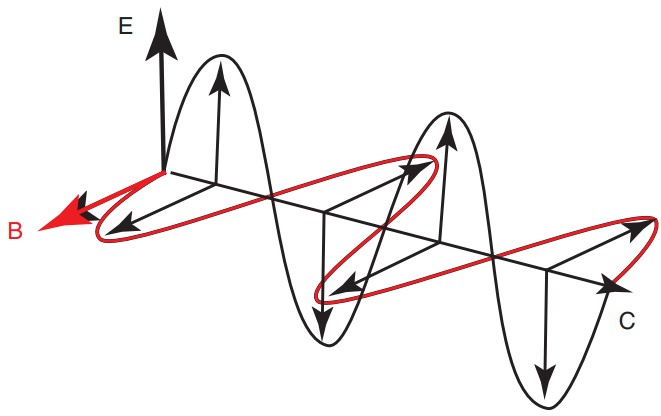
\includegraphics[width=0.6\textwidth]{Imagens/ondaEletromagnetica.jpg}
                        \caption{Propagação da onda eletromagnética}
                        \label{fig:ondaEletromagnetica}
                    \end{figure}
            
            As equações relacionadas ao movimento ondulatório e a energia do fóton são:

            \begin{itemize}
                \item A amplitude da onda é dada por:
                
                    \begin{equation}
                        A = A_0 \sin (2 \pi \nu t)
                    \end{equation}
                    \noindent onde $\nu$ é a frequência de oscilação da onda
                
                \item A frequência $\ni$ e o comprimento de onda $\lambda$ estão relacionados através da equação:
                    
                    \begin{equation}
                        \nu = \frac{c}{\lambda}
                    \end{equation}

                    \noindent onde c é a velocidade da luz no vácuo;

                \item O momento $p$ de um fóton é obtido através da relação:
                
                    \begin{equation}
                        p = h \; \frac{\nu}{c} = \frac{h}{\lambda}
                    \end{equation}

                    \noindent onde $h$ é a constante de Planck.

                \item E energia de um fóton $E$ é dada pela relação:
                
                    \begin{equation}
                        E = h \nu
                    \end{equation}

            \end{itemize}

            Quando se tratam de velocidades próximas a da luz, é importante enfatizar as esquações relativísticas:

            \begin{itemize}
                \item Massa relativística de uma partícula com velocidade $v$
                
                    \begin{equation}
                        m(v) = 
                        \frac{m_0}{\sqrt{1 - \left(\frac{v}{c}\right)^2}} = 
                        \frac{m_0}{\sqrt{1 - \beta^2}} =
                        \gamma m_0
                    \end{equation}

                \item Energia relativística de uma partícula que se move com velocidade $v$:
                    
                    \begin{equation}
                        E = m(v)c^2
                    \end{equation}

                \item Energia de repouso de uma partícula:
                
                    \begin{equation}
                        E_0 = m_0 c^2
                    \end{equation}
                    Para fótons, $E_0 = 0$

                \item Energia Cinética $E_k$ de uma partícula se movendo com $v$:
                
                    \begin{equation}
                        E_k = E - E_0 = (\gamma -1)E_0
                    \end{equation}
                    
                \item Relação entre a energia e o momento da partícula:
                
                    \begin{equation}
                        E^2 = E_0^2 + p^2c^2
                    \end{equation}
            \end{itemize}

            \subsubsection{Espectro Eletromagnético}

                A Figura \ref{fig:espectroEM} mostra a faixa de comprimentos de onda que contemplam o espectro eletromagnético. Em ordem crescente de energia, temos: \textbf{ondas de rádio, micro-ondas, infravermelho, luz visível, raios ultra-violeta, raios-X, raios-gama e raios cósmicos.}

                \begin{figure}[h]
                    \centering
                    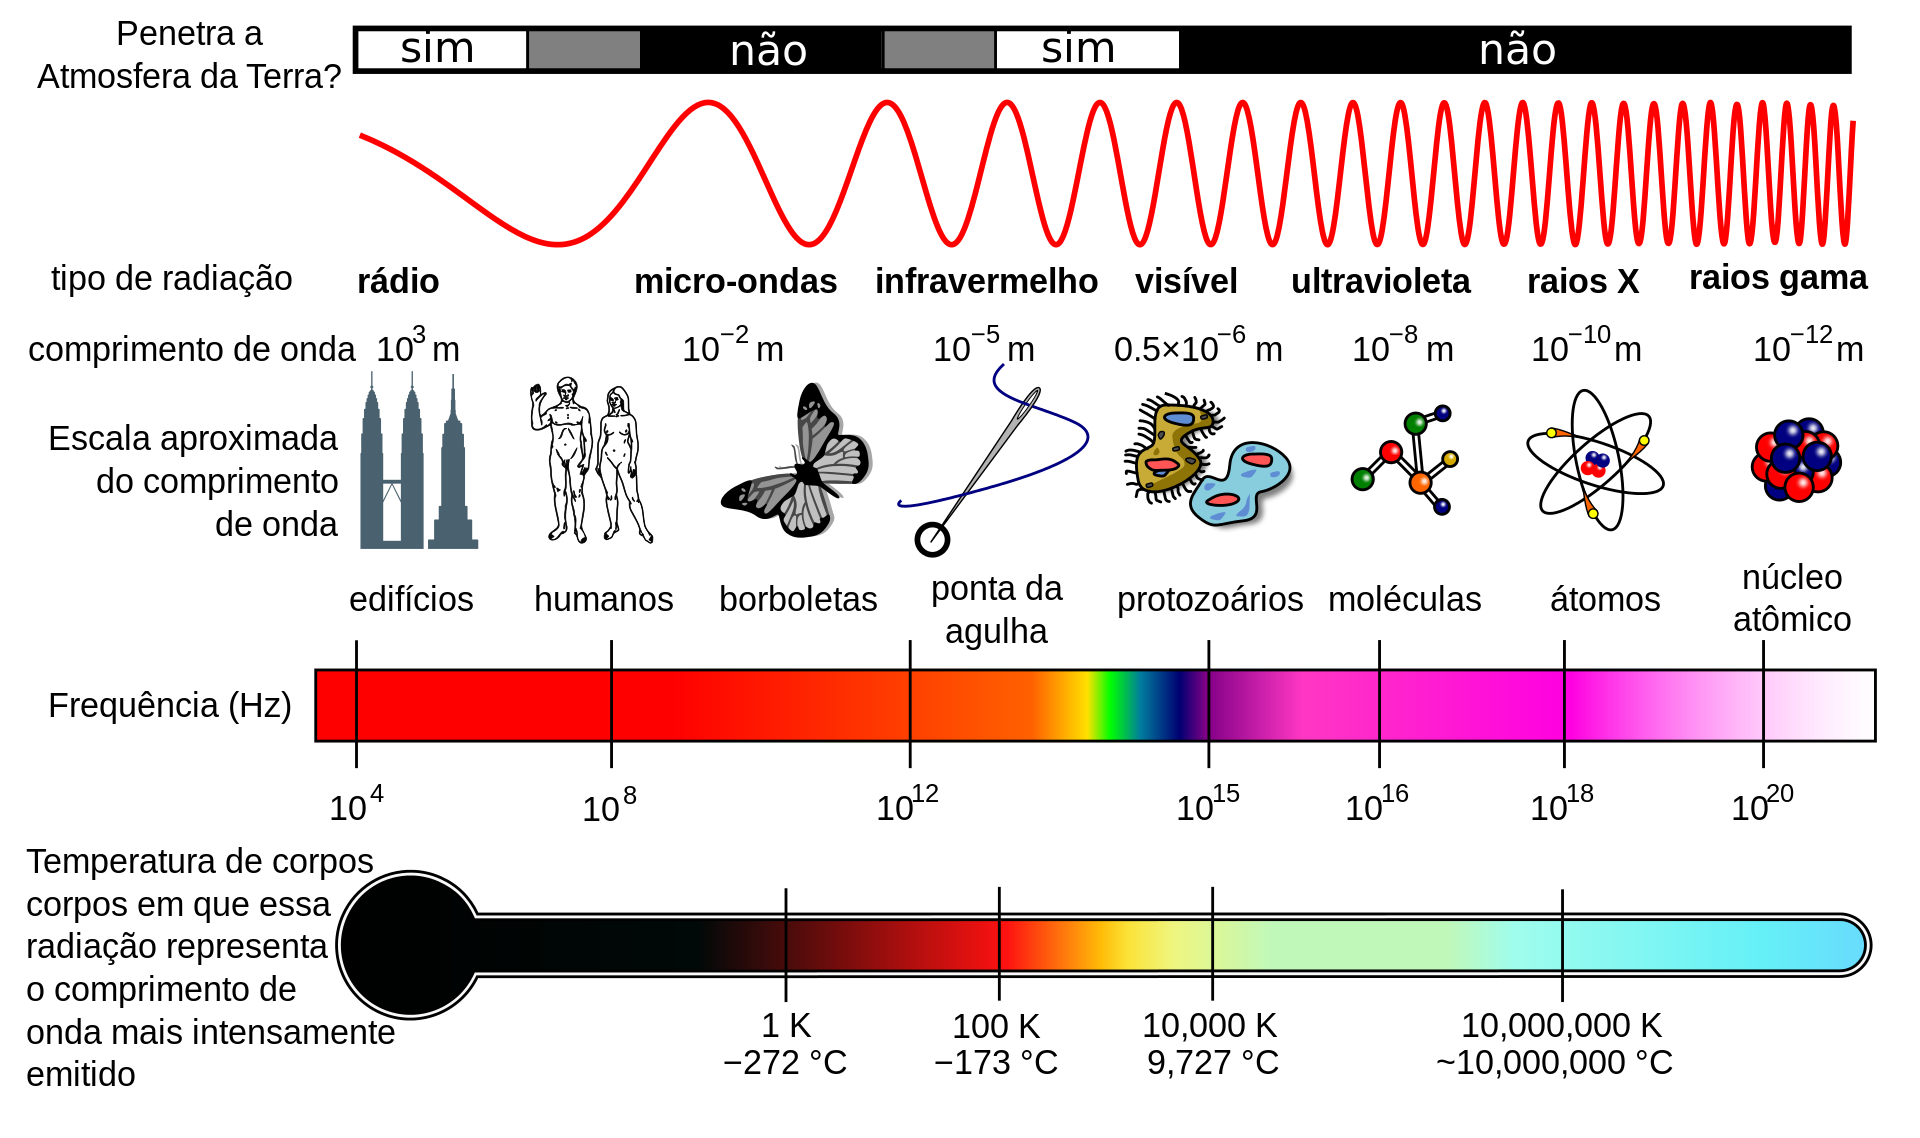
\includegraphics[width=0.7\textwidth]{Imagens/espectroEM.jpg}
                    \caption{Espectro Eletromagnético}
                    \label{fig:espectroEM}
                \end{figure}

                 A menor energia de ligação de um elétron no átomo é de 13.6 eV para um átomo de hidrogênio, e portanto, a radiação EM só tem energia suficiente para causar ionização a partir dos raios UVC. Como os raios-x possuem energia $>$ 124 eV (10 nm), eles possuem energia acima do limiar e portanto podem causar ionizações. Embora a radiação UV não cause ionizações, elas podem causar excitação dos elétrons de valência, alterando as ligações químicas das moléculas; Por isso ocorrem vermelhidão na pele ou alteração da cor da pele devido ao bronzeamento.

        \subsection{Produção de Radiação}
                
            A forma como a radiação é produzida impacta na faixa de energia dos fótons emitidos. A tabela \ref{tab:nomesRadiacaoX} mostra a faixa de energia da radiação-x com suas respectivas aplicações.

                \begin{table}
                    \centering
                    \caption{Nomenclatura das faixas de energias da radiação-x}
                    \label{tab:nomesRadiacaoX}
                    \begin{tabular}{c c c c c}
                        \hline
                        Nome & Energia & Profundidade & Uso & Utilização Atual \\
                        \hline
                        Diagnóstico & \qtyrange{20}{150}{kV} & - & Imagens & Comumente \\
                        Superficial & \qtyrange{50}{200}{kV} & \qtyrange{0}{5}{mm}  & Pele & Raramente \\
                        Orthovoltagem & \qtyrange{200}{500}{kV} & \qtyrange{4}{6}{mm}  & Pele e arcos costais & Raramente \\
                        Megavoltagem & \qtyrange{1}{25}{MV} & \qtyrange{1}{30}{cm}  & Tecidos Profundos & Comumente \\
                        \hline
                        \hline
                    \end{tabular}
                \end{table}
        
            \subsubsection{Tubos de Raios-X}

                São comumente utilizados na formação de imagens, como em Imagens planares, mamografia, tomografias  e etc \dots Em um tubo de raois-x, os elétrons são acelerados em direção a um alvo afim de se produzir radiação de Bremsstrahlung. A Figura \ref{fig:tuboDeRaiosX} mostra o esquema de um tubo de raios-x.

                    \begin{figure}[h]
                        \centering
                        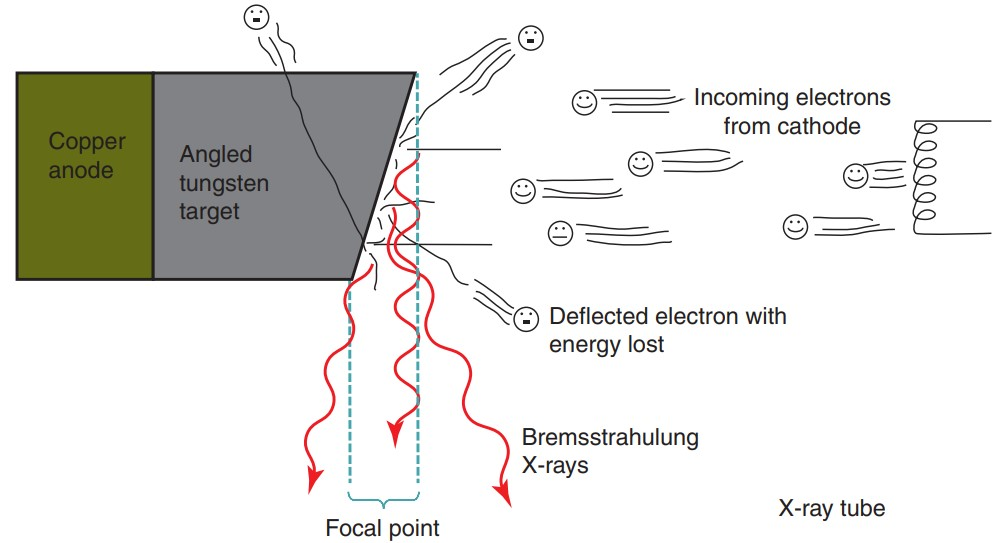
\includegraphics[width=0.7\textwidth]{Imagens/tuboDeRaiosX.jpg}
                        \caption{Tubo de Raios-X}
                        \label{fig:tuboDeRaiosX}
                    \end{figure}
                
                A produção de raios-x se dá da seguinte forma:

                \begin{enumerate}
                    \item Um cátodo, normalmente um filamento feito de tungstênio, é aquecido e libera elétrons através da emissão termoiônica. Estes eletrons flutuam em torno do filamento em uma espécie de nuvem.
                    \item Os elétrons são acelerados no vácuo (para que não colidam com outras moléculas), por um campo elétrico de alta voltagem, medido em kV. 
                    \item Os elétrons são acelerados na direção de um alvo, localizado em frente a um ânodo. Os elétrons são então desacelerados ao colidir com o material do alvo produzindo a radiação de freamento. O material do alvo contem alto número atômico Z e alto ponto de fusão, sendo normalmente de molibdênio ou tungstênio. 
                \end{enumerate}

                O processo de produção de raios-x em um tubo é extremamente ineficiente, de forma que 99\% da energia produzida é convertida em calor. Para dissipar o calor, são utilizados sistemas de resfriamento utilizando água ou óleo, além da inclusão de ânodos giratórios, o que permite que os elétrons colidam em diferentes regiões do ânodo.
                
                Os raio-x são emitidos em varias direções incluindo para dentro do próprio alvo que irá absorver o fóton produzido.Portanto,  o alvo é projetado para ser angulado de forma que a maior parte dos raios-x produzidos sejam direcionados para a janela do tubo, onde será formado o feixe útil. 
                
                O ângulo do alvo afeta a largura do ponto focal por onde emergirá o feixe útil. Para fins de imagens, o ponto focal deve ser o menor possível (\qtyrange{0.3}{3}{mm}), para garantir uma melhor qualidade da imagem, ao mesmo tempo que tenha angulação suficiente para direcionar os raios-x para a direção específica. Uma angulação do alvo entre \ang{7} - \ang{18} é suficiente para criar um pequeno ponto focal onde os raios-x produzidos são emitidos preferencialmente à \ang{90} da direção de propagação dos elétrons incidentes.

                Como os raios-x são formados em diferentes profundidades no alvo, os raios-x produzidos em uma profundidade maior do alvo sofrem mais atenuação quando comparado aos raios-x produzidos na superfície do alvo; Portando há uma maior intensidade de radiação na direção do cátodo que diminui gradativamente na direção do ânodo, esse efeito é conhecido como efeito anódico. Para uniformizar o feixe são utilizados filtros compensadores.


                Existem dois circuitos elétricos no tubo de raios-x, um controla a corrente no filamento que é responsável pelo aquecimento do filamento e controla a emissão termoiônica, e outro controla a tensão no tubo que está relacionada com a energia do fóton emitido e o rendimento.

                A filtração inerente é aquela que atenua o feixe devido aos próprios componentes do tubo. A filtração inerente é medida em mm Linac equivalente e possui valores típicos de \qtyrange{0.5}{1}{mm Linac}. Uma filtração adicional é requerida para filtrar os raios-x de baixa energia produzidos afim de reduzir dose desnecessária no paciente, sendo necessário uma filtragem adicional de no mínimo \qty{2.5}{mm Linac}. Filtros compensadores podem ser utilizados para reduzir altas intensidades do feixe resultantes de exposição em regiões mais finas ou de baixa atenuação, que podem exceder a capacidade do detector. Um exemplo é o filtro bowtie utilizados em imagens de TC.

                A unidade mAs (miliampere-segundo) é uma medida utilizada para controlar a quantidade de radiação produzida por um tubo de raios-X durante a exposição de um paciente. Ela é a multiplicação da corrente elétrica (medida em miliampères - mA) pelo tempo de exposição (medido em segundos - s).

                O valor de mAs é importante porque afeta a quantidade de radiação que é absorvida pelo paciente durante a exposição aos raios-X. Quanto maior o valor de mAs, maior a quantidade de radiação que é produzida pelo tubo de raios-X, resultando em uma imagem mais escura e com mais detalhes. No entanto, também pode aumentar a dose de radiação absorvida pelo paciente.

                A unidade kVp (quilovoltagem pico) é uma medida utilizada para controlar a energia dos elétrons que são acelerados em direção ao ânodo em um tubo de raios-X. A energia dos elétrons é diretamente proporcional à tensão aplicada entre o filamento e o ânodo, que é medida em volts (V).

                O valor de kVp é importante porque afeta a capacidade dos raios-X penetrarem nos tecidos do corpo humano. Quanto maior o valor de kVp, maior a energia dos elétrons e maior a penetração dos raios-X nos tecidos do corpo humano, o que pode ajudar a produzir imagens mais nítidas e detalhadas. No entanto, valores de kVp muito altos podem aumentar o risco de artefatos de imagem e de exposição excessiva à radiação.

                Para tecidos mais densos, como ossos, é comum usar valores mais altos de kVp para permitir que os raios-X penetrem mais profundamente, enquanto valores mais baixos de mAs podem ser usados porque esses tecidos absorvem mais radiação. Para tecidos menos densos, como tecidos moles, são comuns valores mais baixos de kVp para evitar exposições excessivas à radiação, enquanto valores mais altos de mAs podem ser usados para garantir uma boa qualidade de imagem.


            \subsubsection{Radioterapia com Cobalto-60}

                O \ce{^{60}Co} é um radioisótopo produzido em um reator nuclear, que decai para o \ce{^{60}Ni} que emite imediatamente dois fótons com energia de \qty{1.17}{MeV} e \qty{1.33}{MeV} com energia média dos fótons produzidos de \qty{1.25}{MeV} que permite tratar tecidos profundos poupando a pele.
                
                A primeira unidade de \ce{^{60}Co} para tratamento de câncer foi produzida em 1951 e foi amplamente substituída por aceleradores lineares, embora ainda possam ser encontradas em países subdesenvolvidos.

                Atualmente, as fontes de \ce{^{60}Co} ainda são amplamente utilizadas em unidades de GammaKnife. O GK consiste em múltiplas fontes de cobalto inseridas em aberturas que direciona a radiação para um isocentro esférico. O tamanho do isocentro esférico pode ser alterado mudando o tamanho das aberturas da fonte, mas a posição do isocentro não pode ser alterada, portanto para alterar a região de tratamento deve-se movimentar a cabeça em diferentes posições dentro do capacete.

            \subsubsection{Aceleradores Lineares}

                Os Aceleradores Lineares (Linac) só foram desenvolvidos após a Segunda Guerra Mundial, onde foi desenvolvida a tecnologia de micro-ondas de radiofrequência baseadas em partículas aceleradas. 

                Existem duas tecnologias principais utilizadas em aceleradores lineares relacionadas às micro-ondas: Klystron e Magnetron. A figura \ref{fig:esquemaAceleradorLinear} mostra o esquema básico de um Linac clínico.


                \begin{figure}[h]
                    \centering
                    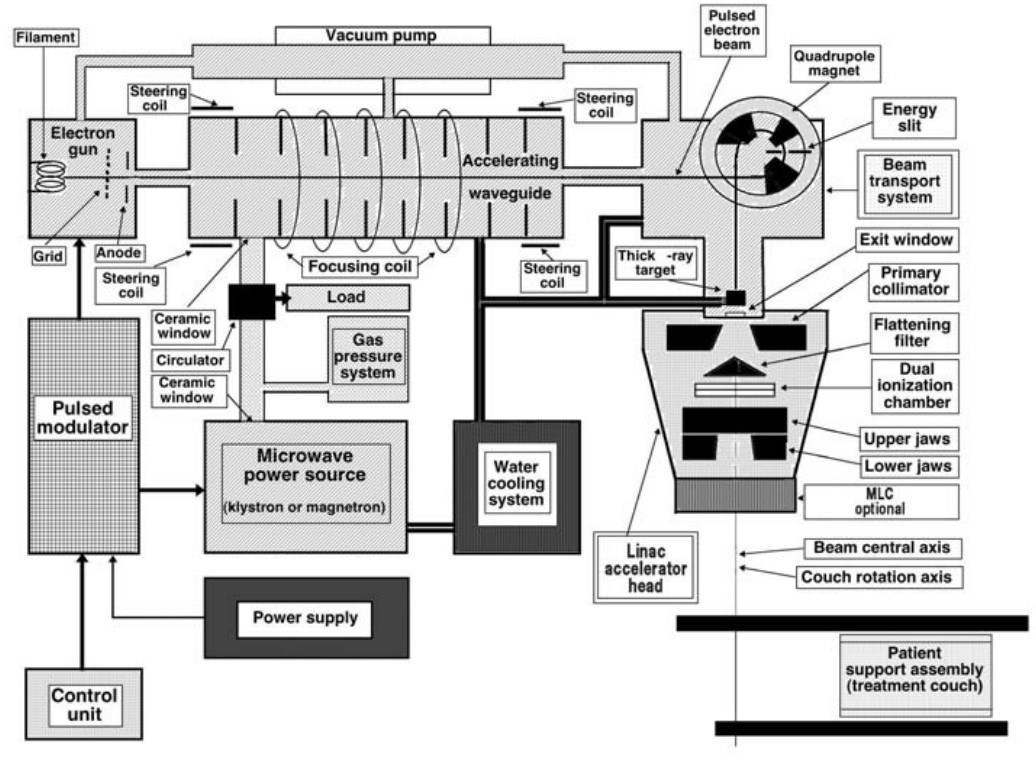
\includegraphics[width=0.7\textwidth]{Imagens/esquemaAceleradorLinear.jpg}
                    \caption{Acelerador Linear Clínico}
                    \label{fig:esquemaAceleradorLinear}
                \end{figure}

            
                A figura \ref{fig:esquemaAceleradorLinear} mostra um esquema geral de um Linac, porém exitem algumas variações significantes entre um fabricante e outro que está relacionada ao design e à energia final dos elétrons acelerados na guia de onda que impacta no tamanho da guia aceleradora. O tamanho da guia aceleradora varia de $\sim $\qty{30}{cm} para $E_k = $ \qty{4}{MeV} até $\sim $\qty{150}{cm} para $E_k = $ \qty{25}{MeV}.

                Os principais componentes de um Linac, responsáveis pela formação do feixe podem ser agrupados nas seguintes classes:

                \begin{enumerate}
                    \item Sistema de injeção;
                    \item Sistema de geração de energia por radiofrequência
                    \item Guia de onda aceleradora
                    \item Sistemas auxiliares
                    \item Sistema de transporte do feixe
                    \item Sistema de monitoramento e colimação do feixe.
                \end{enumerate}
            
            Os fótons produzidos a partir de elétrons com energia da ordem de Megavoltagem são direcionados principalmente na direção de propagação do feixe de elétrons. 
            
            \begin{itemize}
                \item Em uma configuração simples, a gun de elétrons e o alvo fazem parte da guia de onda aceleradora e são alinhados diretamente com o isocentro do Linac evitando a necessidade de um sistema de transporte para o feixe de elétrons. Um feixe de fotons direto é produzido e a fonte de alimentação de RF é montada no Gantry.
                
                \item Este Linac com configuração mais simples é isocentricamente montado para maquinas de \qty{4}{MV} ou \qty{6}{MV}, com a gun de elétrons e o alvo permanetemente embutido na guia de onda aceleradora, não exigindo um sitema de transporte do feixe e nem oferecendo a opção para tratamento com feixes de elétrons.
                
                \item As guias aceleradoras para energias de elétrons intermediárias (\qtyrange{8}{15}{MeV}) e para elétrons com alta energia (\qtyrange{15}{30}{MeV}) são muito longas para serem diretamente montadas alinhadas ao isocentro e portanto são montadas ou no gantry, paralela ao seu eixo de rotação, ou são montadas no suporte do gantry. É utilizado um sistema de transporte do feixe para direcionar o elétron acelerado na guia aceleradora para o alvo. Em ambas configurações, a fonte de alimentação de RF é montada no suporte do gantry. A figura \ref{fig:esquemasMontagemGuia} mostra os diferentes esquemas de montagem da guia de onda.
            \end{itemize}
             

            \begin{figure}[h]
                \centering
                \subfigure[]{\label{fig:AlDireto}
                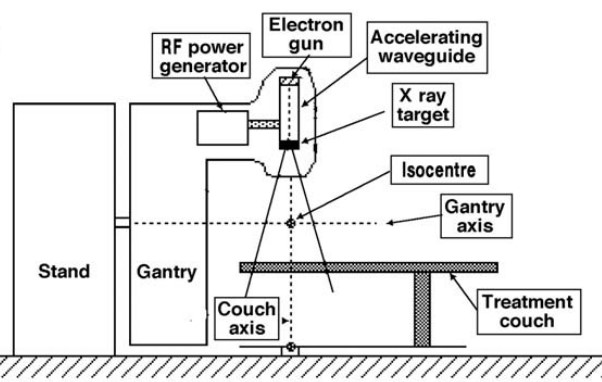
\includegraphics[width=0.4\textwidth]{Imagens/esquemaAceleradorFeixeDireto.jpg}}
                \subfigure[]{\label{fig:AlGuiaNoGantry}
                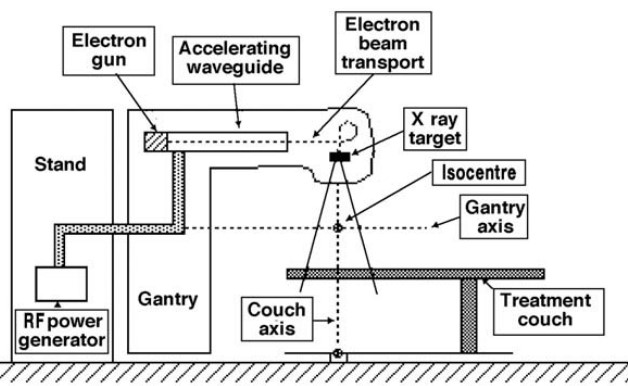
\includegraphics[width=0.4\textwidth]{Imagens/esquemaAceleradorGuiaNoGantry.jpg}}
                \subfigure[]{\label{fig:AlGuiaNoSuporte}
                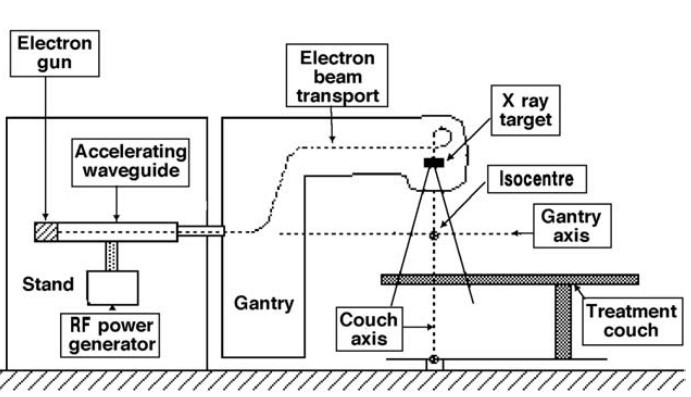
\includegraphics[width=0.4\textwidth]{Imagens/esquemaAceleradorGuiaNoSuporteDoGantry.jpg}}
                \caption{Esquemas de montagem da guia aceleradora em Linacs onde \ref{fig:AlDireto} a guia de onda é montada alinhada ao isocentro do gantry, \ref{fig:AlGuiaNoGantry} a guia de onda é montada paralelamente ao eixo de rotação do gantry e \ref{fig:AlGuiaNoSuporte} a guia de onda é montada no suporte do gantry}.
                \label{fig:esquemasMontagemGuia}
            \end{figure}

                \begin{itemize}
                    \item \textbf{\textit{\textcolor{CarnationPink}{Sistema de Injeção}}}
                \end{itemize}

                    O Sistema de injeção consiste em uma acelerador eletrostático chamado de gun de elétrons.

                    \begin{itemize}
                        \item A gun de elétrons pode ser de dois tipos: Tipo Diodo ou Tipo Triodo.
                        
                        \item Ambos os tipos consistem em um filamento de cátodo aquecido e um ânodo perfurado aterrado e a gun do tipo triodo também possue uma grade incorporada. Os elétrons são  termionicamente emitidos a partir do cátodo aquecido e são focados em um feixe lápis através de eletrodos curvos de foco e então são acelerados em direção ao ânodo perfurado  através do qual eles são impulsionados para entrar na guia aceleradora.
                        
                        \item Os campos eletrostáticos utilizados para acelerar os elétrons na gun do tipo diodo são alimentados diretamente pelo modulador pulsado na forma de um pulso negativo entregue ao cátodo da gun.
                        
                        \item Na gun do tipo triodo, o cátodo é mantido em um potencial estático negativo (normalmente de \qty{-20}{kV}). A grade do triodo é mantida suficientemente negativa em relação ao cátodo para cortar a corrente para o ânodo. A injeção dos elétrons na guia de onda é controlada através de pulsos de voltagem que são aplicados na grade e devem estar sincronizados com os pulsos aplicados no gerador de micro-ondas.
                    \end{itemize}
                    
            
                \begin{itemize}
                    \item \textbf{\textit{\textcolor{CarnationPink}{Sistema de Geração de Energia por Radiofrequência}}}
                \end{itemize}

                    A radiação de micro-ondas utilizadas na guia de onda para acelerar os elétrons até uma energia desejável é produzida por um sistema de geração de radiofrequência, que possui duas componentes principais: Uma fonte de radiofrequência e um modulador pulsado. 

                    \begin{itemize}
                        \item A fonte de RF pode ser ou uma magnetron ou uma klystron. Ambos são dispositivos que utilizam a aceleração e desaceleração do elétron no vácuo para produzir campos de radiofrequência com alta energia. Ambas utilizam os eletrons emitidos por emissão termoionica no cátodo acelerados em direção ao ânodo em um campo eletrostático pulsado, porém utilizam princípios diferentes em seu design.
                        \item A alta voltagem (~ 100 kV), a alta corrente (~ 100 A) e os pulsos de curta duração ( ~1s) necessários para a fonte de RF (Klystron ou Magnetron) são produzidos por um modulador pulsado. O circuito do modulador pulsado está alojado no gabinete do modulador, no qual depende do design de instalação particular do Linac, e fica localizado dentro da sala de tratamento em uma sala mecanica especial ou na sala de controle do Linac.
                        \item A magnetron é uma fonte de radiofrequência de alta energia necessária para a aceleração dos elétrons enquanto que a Klystron é um amplificador de radiofrequência que amplifica as micro-ondas de baixa energia geradas por um oscilador de RF comumente chamado de RF driver. 
                    \end{itemize}

                
                \begin{itemize}
                    \item \textbf{\textit{\textcolor{CarnationPink}{Guias de onda aceleradoras}}}
                \end{itemize}
                 
                    As guias de onda são estruturas metálicas, preenchidas com vácuo ou com um gás, tendo sua seção transversal em formato retangular ou circular. Os Aceleradores Lineares podem utilizar dois tipos de guias de onda: As guias de onda de transmissão de energia de radiofrequência e as guias de onda de aceleração.  As guias de onda de transmissão de RF transmitem as ondas de RF provenientes da fonte de RF para a guia de onda aceleradora. 

                    \begin{itemize}
                        \item Os elétrons são acelerados na guia aceleradora através da transferência de energia dos campos de RF de ata energia, no qual são configuradas na guia aceleradora e produzidas no gerador de RF. 
                        
                        \item O modelo mais simples de uma guia de onda consiste em uma guia de onda cilindrica uniforme contendo uma  série de discos equidistantes (íris) com orifícios circulares em seu centro ao longo de todo o tubo. Estes discos dividem a guia de onda em uma série de cavidades cilindricas que forma a estrutura básica da guia aceleradora do linac. 
                        
                        \item É formado um vácuo dentro da guia aceleradora para permitir a livre propagação dos elétrons.
                        
                        \item As cavidades dentro da guia aceleradora servem para acoplar e distribuir as micro-ondas entre as cavidades adjacentes e para fornecer um padrão de campo elétrico adequado para a aceleração dos elétrons.
                        
                        \item Existem dois tipos de guias aceleradoras: Guia com estrutura de onda progressiva (travelling wave) e guia com estrutura de onda estacionária.
                        
                        \item Na guia de onda que utiliza estrutura de onda progressiva, as micro-ondas entram na guia aceleradora pelo lado da gun de elétrons e propagam em direção à extremidade de alta energia da guia de onda, onde as micro-ondas são absorvidas sem qualquer reflexão ou saem da guia de onda para serem absorvidas por uma carga resistiva ou para ser realimentada na extremidade de entrada da guia aceleradora. Nesta configuração apenas uma em cada quatro cavidades é, em um determinado momento, adequada para a aceleração dos elétrons, fornecendo um campo elétrico na direção de propagação.
                        
                        \item Na guia de onda que utiliza estrutura de onda estacionária, cada extremidade da guia de onda é terminada com um disco condutor para refletir as micro-ondas resultando em um acúmulo de ondas estacionárias na guia de onda. Nesta configuração, em todos os momentos, cada segunda cavidade não carrega campo elétrico e, portanto não produz ganho de energia para os elétrons. Estas cavidades servem apenas como cavidades de acoplamento e podem ser movidas para o lado da estrutura da guia de onda, efetivamente encurtando a guia de onda aceleradora em 50\% do seu tamanho. A Figura \ref{fig:corteGuiaDeOndaEstacionaria} mostra um corte longitudinal de uma guia de onda estacionária.
                    \end{itemize}

                    \begin{figure}[h]
                        \centering
                        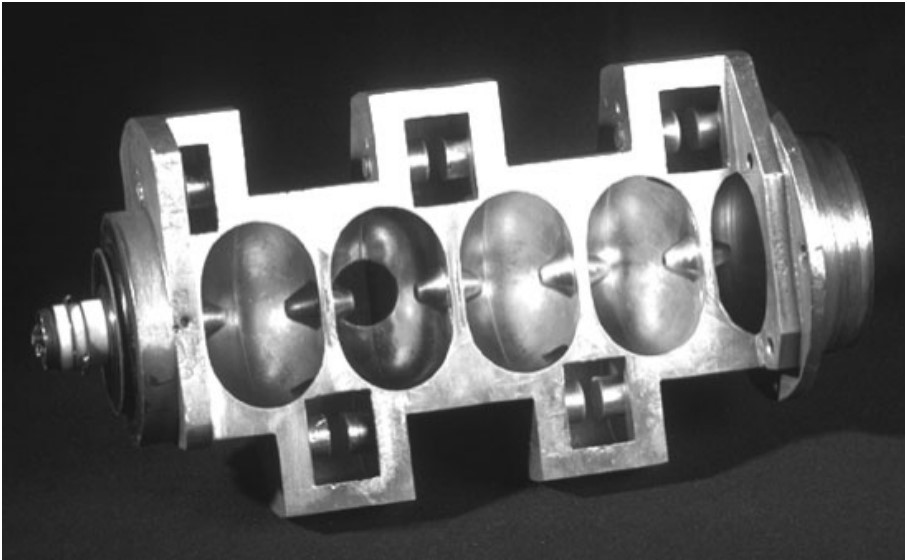
\includegraphics[width=0.7\textwidth]{Imagens/corteGuiaDeOndaEstacionaria.jpg}
                        \caption{Corte de uma guia de onda aceleradora com estrutura de onda estacionária para um acelerador de 6 MV, onde as cavidades aceleradoras estão no eixo central da guia de onda e as cavidades de acoplamento estão lateralizadas na estrutuda da guia. A gun de elétrons está permanentemente fixada na esquerda da guia aceleradora e o alvo está permanentemente fixado na direita da guia}
                        \label{fig:corteGuiaDeOndaEstacionaria}
                    \end{figure}


                \begin{itemize}
                    \item \textbf{\textit{\textcolor{CarnationPink}{Guias de onda aceleradoras}}}
                \end{itemize}


                    As micro-ondas produzidas no gerador de RF são levadas para a guia de onda aceleradora através de guias de ondas retangulares uniformes de banda S que são mantidas no vácuo ou são pressurizadas com um gás dielétrico (Freon ou Hexafluoreto de Enxofre \ce{SF6}) até o dobro da pressão atmosférica.

                    \begin{itemize}
                        \item Um importante componente que deve ser inserido no circuito de transmissão de RF entre o gerador de RF e a guia aceleradora é o circulador, também chamado de isolador, que transmite a micro-onda do gerador de RF para a guia aceleradora ao mesmo tempo que impede a radiação refletida que se move na direção oposta à micro-onda transmitida, protegendo a fonte de RF da energia refletida.
                    \end{itemize}


                \begin{itemize}
                    \item \textbf{\textit{\textcolor{CarnationPink}{Sistemas Auxiliares}}}
                \end{itemize}

                    São aqueles que não estão diretamente envolvidos com a aceleração dos elétrons mas que garantem que a aceleração ocorra e que o Linac se mantenha viavel para utilização clínica. Os sistemas auxiliares são:

                    \begin{itemize}
                        \item Uma sistema contendo uma bomba de vácuo que produz uma pressão de vácuo de ~ 10 torr até 6 torr tanto na guia aceleradora quanto no gerador de RF.
                        \item Um sistema de resfriamento de água utilizado para resfriar a guia aceleradora, o alvo, o circulador e o gerador de RF;
                        \item Um sistema opcional de ar pressurizado utilizado para movimentos pneumáticos do alvo e outros componentes de conformação do feixe;
                        \item Uma blindagem para conter a radiação de fuga.
                    \end{itemize}

                \begin{itemize}
                    \item \textbf{\textit{\textcolor{CarnationPink}{Transporte do Feixe de Elétrons}}}
                \end{itemize}

                    Em aceleradores de baixa energia, o alvo é embutido na guia aceleradore não sendo necessário um sistema de transporte do feixe de elétrons entre a guia e o alvo. Em aceleradores cuja guia de onda não é montada no mesmo sentido da saída do feixe, são utilizados bending magnets para curvarem o feixe de elétrons e direcioná-los para o alvo ou à folha espalhadora. Existem três tipos de bending magnets: 
                    
                        \begin{enumerate}
                            \item Bending de \ang{90};
                            \item Bending de \ang{270} (acromático); e
                            \item Bending de \ang{112.5} (ziguezague)
                        \end{enumerate}

                    O sistema de transporte de elétrons consiste em tubos direcionadores com vácuo, e bendings magnets. Adicionalmente bobinas de direcionamento e bobinas de foco utilizadas para direcionar e focar o feixe de elétrons também fazem parte do sistema de transporte. 

                \begin{itemize}
                    \item \textbf{\textit{\textcolor{CarnationPink}{Cabeçote de Tratamento do Acelerador}}}
                \end{itemize}

                    No cabeçote estão várias estruturas que influenciam na produção, conformação, localização e no monitoramento dos feixes clínicos de fótons e elétrons. O Feixe de elétrons chega no cabeçote na forma de pencil beam para então ser produzidos os feixes clínicos de fótons e elétrons. 

                    Os principais componetes presentes no cabeçote do acelerador são:

                    \begin{enumerate}
                        \item Vários alvos retráteis para a produção de raios-X;
                        \item Filtro aplanador e folha espalhadora;
                        \item Colimadores primários e Colimadores secundários ajustáveis;
                        \item Dupla câmara de ionização de transmissão;
                        \item Luz de campo e telêmetro;
                        \item Filtros retráteis opcionais;
                        \item MLC opcional.
                    \end{enumerate}


                    \begin{itemize}
                        \item Os feixes clínicos de fótons são produzidos através da comninação do alvo com um filtro aplanador.
                        \item Os feixes clínicos de elétrons são produzidos retraindo o alvo e o filtro aplanador da direção do pencil beam e espalhando o pencil beam utilizando uma folha espalhadora simples ou dupla, ou defletindo e mapeando o feixe lápis de elétrons magneticamente para cobrir o tamanho de campo requerido para o tratamento com elétrons. Cones especiais são utilizados para colimar o feixe de elétrons.
                        \item Cada feixe clínico de fótons tem sua própria combinação de alvo e filtro aplanador. Os filtros aplanadores e as folhas espalhadoras são montadas em um carrosel ou em uma gaveta deslizante para facilitar seu posicionamento mecânico na frente do feixe conforme necessário.
                        \item Os colimadores primários definem o campo circular máximo, no qual é posteriormente truncado com colimador retangular ajustável que consistem em dois jaws superiores e dois jaws inferiores, independentes que produzem campos quadrados e retangulares com uma dimensão máxima de \qtyproduct{40 x 40}{cm} no isocentro do acelerador.
                        \item As câmaras de ionização de transmissão são utilizadas para monitorar o output do feixe de fótons e elétrons assim como a planura radial e transversal do feixe.
                        \item A luz de campo e o telêmetro auxiliam no posicionamento do paciente com base nos marcadores de posicionamento inseridos no paciente.
                    \end{itemize}
                    
                \begin{itemize}
                    \item \textbf{\textit{\textcolor{CarnationPink}{Produção de Feixes Clínicos de Fótons No Linac}}}
                \end{itemize}

                    Os feixes clinicos de fótons são produzidos através da colisão dos elétrons com um alvo, e aplanados utilizando um filtro aplanador. Quando um feixe de fótons atravessa o colimador primário, ele tende a ser muito intenso em seu centro e menos intenso em sua periferia. Portanto o filtro aplanador torna o feixe uniforme (plano) no isocentro. Porém, alguns equipamentos, possuem a opção de remover o filtro aplanador, para que esta característica do feixe possa ser utilizada propositalmente em tratamentos de SBRT, por exemplo.
                    
                    Para feixes produzidos com elétrons com energia abaixo de \qty{15}{MeV} o alvo ideal deve possuir alto número atômico, já os feixes produzidos com elétrons com energia superior a \qty{15}{MeV} o material ideal do alvo deve ter um baixo número atômico. O material do filtro aplanador deve possuir baixo Z independente da energia do feixe.

                    A maior parte dos AL's utilizam o tungstênio como material do alvo devido ao seu alto número atômico (Z = 74) que favorece a produção de raios-x de bremsstrahlung e possuir alto ponto de fusão (\qty{3422}{\degreeCelsius}).

                    

                \begin{itemize}
                    \item \textbf{\textit{\textcolor{CarnationPink}{Colimação do Feixe}}}
                \end{itemize}

                    Em um sistema de colimação existe o colimador primário, que é fixo; o colimador secundário, composto por jaws móveis e por um colimador terciário opcional, chamados de Multileaf colimator; Nos feixes de eletrons, são utilizados, adicionalmente, aplicadores.

                    \begin{itemize}
                        \item O colimador primário define o maior tamanho de campo circular possível. E modelado em um formato cônico utilizando uma blindagem de tungstênio, com os lados da abertura cônica projetando-se nas bordas do alvo em uma extremidade do bloco e no filtro de nivelamento na outra extremidade. A espessura da blindagem é determinada de modo que atenue a intensidade média do feixe primário que sai do cabeçote para menos de 0.1\% da intensidade incial do feixe primário.
                        
                        \item Os colimadores secundários são responsáveis por definir o tamanho de campo de tratamento e consiste em quatro blocos divididos em 2 jaws superiores de 2 jaws inferiores, que formam campos quadrados ou retangulares variando de poucos milímetros até \qty{40}{cm}.
                        
                        \item Aceleradores mais antigos, tem a movimentação dos jaws ocorrendo simetricamente, (cada jaw abre o mesmo tamanho a partir do isocentro). Aceleradores mais modernos possuem jaws assimétricos, onde a movimentação de cada jaw é feita independentemente, permitindo utilizar campos assimétricos como os campos meio-bloqueados.
                        
                        \item O MLC está relacionado a terapia conformacional, sendo utilizados nas técnicas de intensidade modulada, com step and shoot, dmlc, ou terapia com arco.
                        
                        \item Os micro-multileaf são projeados com lâminas com espessuras finas no isocentro, abrindo campos da ordem de \qtyproduct{10 x 10}{cm} para serem utilizados em tratamentos de radiocirurgia.
                    \end{itemize}

                \begin{itemize}
                    \item \textbf{\textit{\textcolor{CarnationPink}{Produção de Feixes Clínicos de Elétrons No Linac}}}
                \end{itemize}

                Para habilitar o modo feixe de elétrons, o alvo e o filtro aplanador são removidos do caminho do feixe de elétrons. A corrente dos feixes de elétrons produzidos em feixes clínicos são de duas a três ordens de magnetude menores que aquelas utilizadas na produção de feixes clínicos de fótons. O feixe lápis de elétrons sai do sistema de transporte à vacuo do feixe através de uma fina janela, normalmente feita de Berílio (\ce{Be}), no qual possui um baixo número atômico, o que minimiza o espalhamento do feixe e a produção de raios-x Bremsstrahlung.

                    \begin{itemize}
                        
                        \item Existem duas técnicas possíveis na produção do feixe clínico de elétrons a partir do feixe lápis:
                        
                            \begin{enumerate}
                                \item \textbf{Espalhamento do Feixe lápis}: O espalhamento do feixe lápis (que possui área de ~ \qty{4}{mm^2})  em uma área alargada, fornecendo tamanhos de campo de até \qtyproduct{25 x 25}{cm} é alcançado colocando finas folhas feitas em material com alto número atômico (cobre ou chumbo) na frente do feixe lápis, no nível do filtro aplanador utilizados no modo fótons. As folhas espalhadoras modificam o feixe fino alterando o ângulo médio de espalhamento tornando o feixe mais difuso e absorvem a energia dos elétrons incidente e alargam o espectro do feixe lápis. O grau de difusão depende da energia do feixe incidente e do número atômico (Z) do material difusor. Por isso, uma única folha difusora não consegue garantir o espalhamento idealmente para todas as faixas de energia produzidas pelo acelerador linear. A melhor solução consiste na utilização de duas folhas espalhadoras distintas. A primeira folha produz uma difusão básica do feixe enquanto a segunda folha se encarrega de produzir a difusão final esperada para a obtenção de campos homogêneos na faixa de 5cm x 5cm a 30cm x 30cm. Uma folha espalhadora de baixo número atômico não difunde o feixe suficientemente e, em contrapartida, também não o contamina muito com fótons de bremsstrahlung nem degrada muito seu espectro de energia. Uma folha difusora de alto número atômico pode difundir o feixe além do necessário; em contrapartida, pode aumentar a contaminação com fótons de bremsstrahlung além de degradar em demasia o seu espectro de energia. A solução para tudo isso é a utilização de um material de número atômico médio: o Alumínio. Um sistema de duas folhas de alumínio produzirá, satisfatoriamente, feixes extensos e homogêneos, com uma produção mínima de contaminação por fótons e uma degradação mínima do espectro de energia. 
                                

                                \item \textbf{Mapeamento do Feixe lápis}: É uma alternativa às folhas espalhadoras, embora menos utilizada. Esta técnica utiliza dois imãs computadorizadamente controlados chamados de dispositivos eletrônicos de varredura, que defletem o feixe lápis em dois planos ortogonais, mapeando o feixe em toda a largura de campo requerida para o tratamento.  O feixe fino produz um campo extenso por um movimento de varredura bidimensional sincronizado, criado por campos magnéticos variáveis, posicionados após a janela de saída do feixe de elétrons. No sistema de varredura, o feixe extenso é obtido por uma varredura de grande amplitude que produzirá um feixe homogêneo para toda a variedade de campos utilizados. Além disso, a intensidade do campo magnético variará de acordo com a energia nominal do feixe de elétrons utilizado. A contaminação por fótons é mínima nesse processo, pois o feixe primário não colide diretamente com nenhuma folha difusora. Existe, entretanto, uma produção de fótons em segundo grau, causada pelos elétrons que atingem as bordas do colimador, a superfície interna dos cones aplicadores e outras estruturas adjacentes.
                            \end{enumerate}

                        \item O sistema de varredura bidimensional foi abandonado e hoje em dia todos os fabricantes de aceleradores lineares utilizam um sistema de dupla folha espalhadora de alumínio, – uma primária fixa e uma secundária, que varia para cada energia dos feixes clínicos de elétrons, uma vez que Os campos obtidos com dupla folha espalhadora possuem as mesmas características dos obtidos com um dispositivo de varredura e O dispositivo de varredura é um sistema eletrônico razoavelmente complexo que encarece bastante o custo total do equipamento além de estar sujeito a falhas e defeitos de funcionamento quando além de estar sujeito a falhas e defeitos de funcionamento quando além de estar sujeito a falhas e defeitos de funcionamento quando comparado à simplicidade do uso de folhas difusoras de alumínio.
                        
                    \end{itemize}
                

                \begin{itemize}
                    \item \textbf{\textit{\textcolor{CarnationPink}{Sistema De Monitoramento De Dose}}}
                \end{itemize}

                    Os monitores de radiação utilizados nos Aceleradores Lineares clínicos possue um padrão para o tipo de detector que deve ser utilizado, exibição das unidades monitoras, interrompimento da radiação e monitoramento da planura e da taxa de dose, ambos definidos pela IEC 60601-2-1.

                    \begin{itemize}
                        \item As câmaras de ionização mais utilizadas são de transmissão, incorporadas no acelerador na frente do feixe de fótons e elétrons, monitorando continuamente o output do feixe durante o tratamento.
                        
                        \item Normalmente são utilizadas câmaras seladas para manter sua resposta independente da temperatura e pressão do ambiente;
                        
                        \item As câmaras são posicionadas entre o filtro aplanador ou folha espalhadora e o sistema de colimação secundário;
                        
                        \item Por questões de segurança do paciente, o sistema de dosimetria dos AL's consistem em duas câmaras de ionização (primária e secundária) independentes , tanto na sua fonte de alimentação de polarização quanto no eletrômetro de leitura. As duas câmeras são projetadas de forma que caso uma falhe durante o tratamento, a segunda câmara irá terminar a irradiação, usualmente depois de uma dose adcional de apenas poucos por centro acima da dose prescrita foi entregue.
                        
                        \item No caso de falha simultânea das câmaras, o temporizador do AL irá desligar a máquina com uma overdose mímima para o paciente.
                        
                        \item Os principais requisitos para as câmaras de ionização monitoras são:
                        
                            \begin{enumerate}
                                \item Devem tem um efeito mínimo nos feixes clínicos de fótons e elétrons;
                                \item Devem ter resposta independente das condições ambientais de temperatura e pressão;
                                \item Devem operar em condições de saturação;
                            \end{enumerate}
                        
                        \item A câmara de ionização primária mede MU's. Normalmente sua sensibilidade é ajustada de forma que 1 MU corresponde a dose de \qty{1}{cGy} entregue em um phantom de água na profundidade de dose máxima no eixo central do feixe quando é irradiado com um campo de \qtyproduct{10 x 10}{cm} a uma distância da fonte até a superfície (SSD) de \qty{100}{cm}.
                        
                        \item Uma vez que as MU's de tratamento são definidas, após serem alvançadas, o circuito da câmara primária irá terminar a entrega de dose do paciente. E antes de uma nova irradiação, o display das MU's deve ser resetado para o valor zero e uma nova irradiação será possível definindo um novo valor de MU;
                        
                        \item Além das MU's, o sistema de monitoramento de dose também monitora outros parâmetros como simetria, planura e energia do feixe; A medida destes valores requer que os eletrodos das câmaras de ionização primária e secundária sejam divididos em vários setores, com seus sinais resultantes destas medidas devem ser utilizados em circuitos de realimentação automátícos para direcionar o feixe de elétrons através da guia aceleradora, sistema de transporte e alvo ou folha de espalhamento afim de garantir a simetria e planura do feixe.
                        
                        \item Os AL's devem ser equipados com um sistema de monitoração que mostra continuamente a taxa de dose no isocentro e interrompe o feixe quando a medida da taxa de dose excede duas vezes o valor máximo especificado pela descrição técnica da máquina.
                    

                    \end{itemize}
            
            \subsubsection{Microton}

                \begin{wrapfigure}{r}{0.45\textwidth}
                    \centering
                    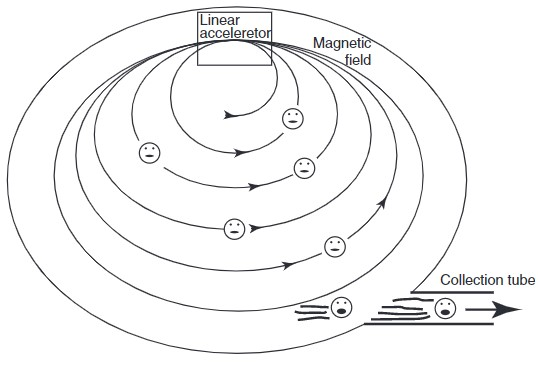
\includegraphics[width=0.4\textwidth]{Imagens/microton.jpg}
                    \caption{Mícroton}
                    \label{fig:microton}
                \end{wrapfigure}
                    
                O mícroton foi inventado no mesmo período que o AL e utilizado em rotinas clínicas na decada de 70, porém a utilização de Al's foi mais aceita por ser mais simples. Um mícroton consiste em um acelerador linear, acoplado a um campo magnético,  onde os elétrons acelerados percorrem uma trajetória circular e entram novamente no acelerador linear ganhando mais velocidade. A figura \ref{fig:microton} mostra o esquema de um mícroton. 
                
                O Loop é controlado pelo campo magnético e a cada vez que o elétron passa no acelerador linear,  ganha energia e portanto o raio do loop aumenta.  É possível produzir eletrons com energia de até \qty{1500}{MeV} e ao alcançar a energia desejada, os elétrons são capturados em um tubo coletor que está associado ao raio do loop.


                Outra forma de mícroton e chamado de \textit{racetrack} onde são utilizadas linhas retas com bending magnets nos finais da tragetória que curvam o feixe de elétrons na forma de uma "pista de corrida"
                


            \subsubsection{Cíclotron}


            \begin{wrapfigure}{l}{0.42\textwidth}
                \centering
                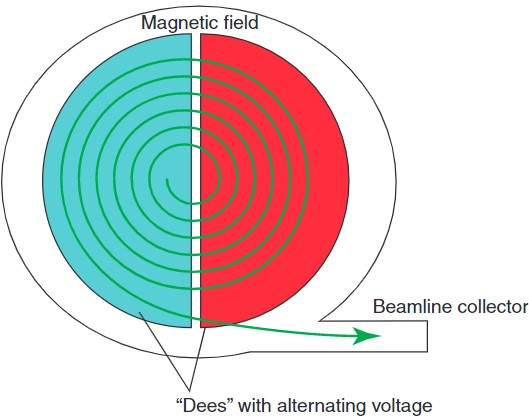
\includegraphics[width=0.4\textwidth]{Imagens/ciclotron.jpg}
                \caption{Cíclotron}
                \label{fig:ciclotron}
            \end{wrapfigure}


                A Figura \ref{fig:ciclotron} mostra um esquema de um Cíclotron que consiste em dois eletrodos em forma de ``D'' com voltagem alternada na presença de um campo magnético perpendicular estático.

                A frequência de alteração da polaridade deve ser combinada com a ``frequência de ressonância do cíclotron'' da partícula alvo permitindo que a partícula desenvolva uma tragetória espiral, ganhando velocidade e massa relativística em cada revolução até que ela colida na parede ou seja coletada no tubo do feixe. 

                Este acelerador pode ser utilizado para acelerar qualquer partícula carregada utilizada em feixes da radioterapia e foi principalmente utilizado para acelerar prótons. 

            \subsubsection{Síncroton}

                Um síncrotron é um acelerador de partículas circular que utiliza campos magnéticos para manter as partículas carregadas em uma trajetória espiralada. As partículas são aceleradas por meio de campos elétricos em um tubo de vácuo e, em seguida, são injetados em um anel de armazenamento, onde são mantidos em uma trajetória circular por meio de ímãs supercondutores.

                Enquanto um cíncroton utiliza um campo magético constante que se alterna com uma frequência constante, o sincroton utiliza um campo magnético com frequência variável que se adapta às mudanças na massa da partícula a cada segmento a medida que a partícula se aproxima da velocidade da luz;

                A estrutura de um síncontron se assemelha a um toróide com segmentos magnéticos que eventualmente alimentam um anel de armazenamento com a linha de feixe útil que posteriormente sai tangenciando o anel de armazenamento externo. 

                A medida que a espiral se torna mais larga e os imãs se tornam mais poderosos, as partículas podem atingir energias extremamente altas (da ordem de GeV) e por isto são utilizados na Radioterapia para acelerar prótons e outras partículas pesadas. 
                
    \section{Interação da Radiação Eletromagnética Com a Matéria}

        Como os fótons não possuem carga, são radiações indiretamente ionizantes e possuem diferentes predominâncias em seus processos de interação, que dependem da energia do fóton e em alguns casos, do número atômico do material com o qual a radiação interage. As interações consiste em três principais mecanismos, a \textbf{\textit{\textcolor{CarnationPink}{absorção}}}, que consiste na dimunuição do número de fótons do feixe devido à absorção da energia desses fótons pelo meio, e o \textbf{\textit{\textcolor{CarnationPink}{espalhamento}}}, que consiste na diminuição do número de fótons do feixe devido à mudança de direção destes fótons. Ao dizer que o feixe sofreu uma \textbf{\textit{\textcolor{CarnationPink}{atenuação}}}, significa que esse feixe diminuiu seu número de fótons devido absorção ou espalhamento.


        \subsection{Atenuação do Feixe de Fótons}

            A intensidade $I(x)$ para um feixe estreito monoenergético de fótons, atenuado por uma espessura de material atenuador $x$ é dado por:

                \begin{equation}
                    I(x) = I_0 e^{-\mu x}
                \end{equation}
            
            \noindent onde $I_0$ é a intensidade inicial do feixe não atenuado e $\mu$ é o coeficiente de atenuação linear que depende da energia do fóton incidente e o número atômico do materaial atenuador.

            O coeficiente de atenuação linear é uma medida da taxa na qual a intensidade de um feixe de radiação é reduzida ao passar por um material. É uma medida da capacidade do material de absorver, espalhar e dissipar a radiação em diferentes direções enquanto ela atravessa o material. Quanto maior o coeficiente de atenuação linear, mais rápida é a taxa de atenuação da radiação, o que significa que o material tem uma maior capacidade de absorver e dispersar a radiação.

            A Camada Semi-Redutora (HVL) é definida como a espessura do material atenuador necessária para atenuar a intensidade do feixe de fótons até 50\% do seu valor original, e pode ser obtida através da relação:

                \begin{equation}
                    x_{1/2} = HVL = \frac{\ln 2}{\mu}
                \end{equation}
            

            A Camada Deci-Redutora é definida como a espessura necessária de material atenuador para atenuar a intensidade do feixe para 10\% do seu valor inicial, e pode ser obtida através da relação:

                \begin{equation}
                    x_{1/10} = TVL = \frac{\ln 10}{\mu}
                \end{equation}

            A relação entre a TVL e a HVL é dada por:

            \begin{equation}
                TVL = \frac{\ln 10}{ \ln 2} HVL = 3.33 HVL
            \end{equation}

            O livre caminho médio $\bar{x}$ é a distância média que um fóton com energia $h \nu$ viaja através de um material absorvedor antes de sofrer uma iteração.  A relação entre o $\bar{x}$ e o coeficiente de atenuação linear $\mu$ é dada pela definição básica de livre caminho médio:

            \begin{equation}
                \bar{x} = \frac{\int_{0}^{\infty} x e^{- \mu x} \,dx }{\int_{0}^{\infty} e^{- \mu x} \,dx } = 
                \frac{\frac{1}{\mu^2}}{\frac{1}{\mu}} = \frac{1}{\mu}
            \end{equation}

            \noindent ou

                \begin{equation}
                    I(x) = \frac{1}{e}I_0 = I_0 e^{-\mu \bar{x}}
                \end{equation}

            \noindent resultando em

                \begin{equation}
                    \frac{1}{e} = e^{-\mu \bar{x}} \quad ou \quad \mu \bar{x} = 1 \quad e \quad \bar{x} = \frac{1}{\mu}
                \end{equation}

            O fator de homogeneidade do feixe de fótons $\chi $ é dado pela razão entre a primeira HVL ($HVL_1$) e a segunda HVL ($HVL_2$),  que é a espessura de material que reduz o feixe de $0.5I_0$ para $0.25I_0$.

                \begin{equation}
                    \chi = \frac{HVL_1}{HVL_2}
                \end{equation}

                \begin{itemize}
                    \item Quando $\chi = 1$ significa que  
                    
                        $$HVL_1 = HVL_2$$ 
                    
                    \noindent Se trata de feixe de fótons monoenergéticos, como o feixe de \ce{^{60}Co} com energia de \qty{1.25}{MeV} e o feixe de \ce{^{137}Cs} com energia de \qty{0.662}{MeV}
                    
                    \item Quando $\chi \neq  1$, os fótons apresentam um espectro de energia. 
                    
                    Caso $\chi <  1$, temos que

                        $$\frac{HVL_1}{HVL_2} < 1 \quad \Rightarrow \quad HVL_1 < HVL_2$$
                        

                    \noindent O que mostra que após a primeira camada semi-redutora, é necessario uma espessura maior para atenuar o feixe em 50\% do seu valor. Neste caso o absorverdor promove o endurecimento do feixe, removendo os fótons de baixa energia do espectro (região do efeito fotoelétrico) 

                    Caso $\chi >  1$, temos que

                        $$\frac{HVL_1}{HVL_2} > 1 \quad \Rightarrow \quad HVL_1 > HVL_2 $$
                        

                    \noindent o que mostra que após a $HVL_1$ é necessário uma menor espessura para atenuar o feixe em 50\% do seu valor. Ocorre então a suavização do feixe na primeira HVL, devido a remoção dos fótons de alta energia do espectro (região da produção de pares).

                \end{itemize}

            Além do coeficiente de atenuação linear $\mu$ são definidos outros coeficientes, também chamados de seção de choque, que definem as características da atenuação do feixe e a relaciona com a probabilidade de ocorrência das interações. 

            O \textbf{\textit{\textcolor{CarnationPink}{Coeficiente de Atenuação Mássico}}} ($\mu_m$) é dado pelo coeficiente de atenuação linear dividido pela massa por unidade de volume do absorvedor ($\rho$ - densidade mássica):

                \begin{equation}
                    \mu_m = \frac{\mu}{\rho}
                \end{equation}

            \noindent onde $\rho$ é a densidade mássica do material absorvedor. A unidade no SI é \unit{m^2/Kg} e quando utilizada nos cálculos, a espessura é obtida em \unit{Kg/m^2}.

            O \textbf{\textit{\textcolor{CarnationPink}{Coeficiente de Atenuação Atômico}}} (${}_a\mu$) é dado pelo coeficiente de atenuação linear dividido pelo número de átomos $N_a$ por volume $\mathcal{V}$ do absorvedor:

                \begin{equation}
                    {}_a\mu = \frac{\mu}{\frac{N_a}{\mathcal{V}}}
                \end{equation}

            \noindent A unidade do SI para o ${}_a\mu$ é \unit{m^2/atomo} que equivale a \qty{e4}{cm^2/atomo}. Quando o ${}_a\mu$ é utilizado na equação de atenuação, a espessura é obtida em \unit{atomo/m^2} onde \qty{1}{atomo/m^2} equivale a \qty{e-4}{atomo/cm^2}


            O \textbf{\textit{\textcolor{CarnationPink}{Coeficiente de Atenuação Eletrônico}}} (${}_e\mu$) é dado pelo coeficiente de atenuação linear dividido pelo número de elétrons $N_e$ por unidade de volume $\mathcal{V}$ do absorvedor.

            \begin{equation}
                {}_e\mu = \frac{\mu}{\frac{N_e}{\mathcal{V}}}
            \end{equation}

            \noindent A unidade do SI para o ${}_e\mu$ é \unit{m^2/eletron}.

            Como ambos os coeficientes são dados em termos da área do material, também são referidos como seção de choque. As relações entre os coeficientes de atenuação são:

            \begin{equation}
                \mu = \rho \mu_m = n\;{}_a\mu = Zn\;{}_e\mu
            \end{equation}

            \noindent onde 

                \begin{equation}
                    n = \frac{N_a}{\mathcal{V}}
                \end{equation}

            \noindent e

                \begin{equation}
                    \frac{N_a}{\mathcal{V}} = \rho \frac{N_a}{m} = \rho \frac{N_A}{A}
                \end{equation}

            Para fins de dosimetria, são definidos outros dois coeficientes de atenuação:

            \begin{enumerate}
                \item \textbf{\textit{\textcolor{CarnationPink}{Coeficiente Linear de Transferência de Energia}}}: Coeficiente utilizado para definir a energia média transferida ($\bar{E}_{tr}$) pelos fótons para as partículas carregadas no meio em uma interação fóton-átomo. É dado por:
                
                    \begin{equation}
                        \mu_{tr} = \mu \frac{\bar{E}_{tr}}{h \nu} = \mu \bar{f}_{tr}
                    \end{equation}

                \noindent onde $\bar{f}_{tr}$ é a fração média total da energia do fóton que é transferida na forma de energia cinética para partículas carregadas através de várias interações entre o fóton incidente e o material do absorvedor.
                
                \item \textbf{\textit{\textcolor{CarnationPink}{Coeficiente Linear de Absorção de Energia}}}: Coeficiente utilizado para definir a energia média absorvida ($\bar{E}_{ab}$)pelo meio em uma interação fóton-átomo. É dado por:
                    
                    \begin{equation}
                        \mu_{ab} = \mu \frac{\bar{E}_{ab}}{h \nu} = \mu \bar{f}_{ab}
                    \end{equation}

                \noindent onde $\bar{f}_{ab}$ é a fração média total da energia do fóton que é absorvida pelo material absorvedor.
            \end{enumerate}

            A energia média transferida por um fóton para uma partícula carregada do meio pode ser definida através da soma de duas componentes: A energia média absorvida pelo meio absorvedor ($\bar{E}_{ab}$) e a energia média perdida pelas partículas carredas secundárias irradiada em forma de radiação eletromagnética, podendo ser radiação de bremsstrahlung, aniquilação em voo ou produção fluorescente devido a desexitação do átomo ($\bar{E}_{rad}$).
            
                \begin{equation}
                    \bar{E}_{tr} = \bar{E}_{ab} + \bar{E}_{rad}
                \end{equation}

            \noindent o que nos permite chegar na relação:

                $$\frac{\mu_{ab}}{\rho} = \frac{\bar{E}_{tr} - \bar{E}_{rad}}{h \nu} \frac{\mu}{\rho} = \frac{\mu_{tr}}{\rho} \left(1 - \frac{\bar{E}_{rad}}{\bar{E}_{tr}}\right) = \frac{\mu_{tr}}{\rho} (1 - \bar{g}) $$

                \begin{equation}
                    = \frac{\mu}{\rho}\bar{f}_{tr}(1 - \bar{g}) = \frac{\mu_{tr}}{\rho}(1 - \bar{g})
                \end{equation}

            \noindent onde $\bar{g}$ é a fração média de radiação definida como a fração da energia cinética média transferida do fóton incidente para a partícula carregada do meio que é subsequentemente irradiada na forma de fótons.

                \begin{equation}
                    \bar{g} = \frac{\bar{E}_{rad}}{\bar{E}_{tr}} 
                    = 1 - \frac{\bar{E}_{ab}}{\bar{E}_{tr}}
                    = 1 - \frac{\bar{f}_{ab}}{\bar{f}_{tr}}
                    = 1 - \frac{\mu_{ab}/ \rho}{\mu_{tr}/ \rho}
                \end{equation}

                
            Em um feixe largo, além do feixe primário, devem ser considerados os os fótons secundários que são espalhados no meio absorvedor e que contribui nos na energia transferida para o meio avaliada na área de abrangência do campo de radiação, diferentemente do feixe estreito que a radiação é espalhada para outra região diferente daquela no qual o feixe primário está incidindo. 

                \begin{equation}
                    B = \frac{I_B(x)}{I_N(x)} 
                \end{equation}

            \noindent onde $B$ é o fator de build-up que representa os fótons secundários que são espalhados, $I_N(x)$ é a intensidade para um feixe estreito e $I_B(x)$ é a intensidade para o feixe secundário. Portanto

                \begin{equation}
                    I_B(x) = I_{N_0} e^{- \bar{\mu}_{eff} x}
                \end{equation}

            \noindent onde

                \begin{equation}
                    \bar{\mu}_{eff} = \mu - \frac{\ln B}{x}
                \end{equation}




        \subsection{Espalhamento Coerente (Rayleigh, Thompson)}

            Este processo de interação ocorre nas faixas de energia de \qtyrange{1}{1000}{keV} onde $h\nu \ll m_ec^2$, Figura \ref{fig:espalhamentoCoerente}. Ao interagir com um elétron orbital fracamente ligado (com ação combinada do átomo inteiro), este fóton é absorvido pelo elétron que começa a oscilar em alta frequência (oscilação de dipolo induzida), e ao relaxar, este excesso de energia é liberado como outro fóton com a mesma energia do fóton incidente porém com uma pequena angulação em relação a tragetória do fóton incidente. Como nenhuma energia é transferida, este espalhamento não contribui para o coeficiente de transferencia de energia, porém contribui para o coeficiente de atenuação, além do mais, este efeito não causa ionizações e portanto não contribui para a dose absorvida no meio.

            \begin{itemize}
                \item A secão de choque atômica para o Espalhamento coerente é proporcional a:  ${}_a\sigma_R \propto (z / h\nu)^2$
                \item O coeficiente de atenuação mássico é proporcional a: $\mu_R / \rho \propto (z / h\nu)^2$
            \end{itemize}

            No tecido e em materiais tecido-equivalentes, a importancia relativa do espalhamento coerente é pequena, contribuindo com poucos \% do coeficiente de atenuação total;

            \begin{figure}[h]
                \centering
                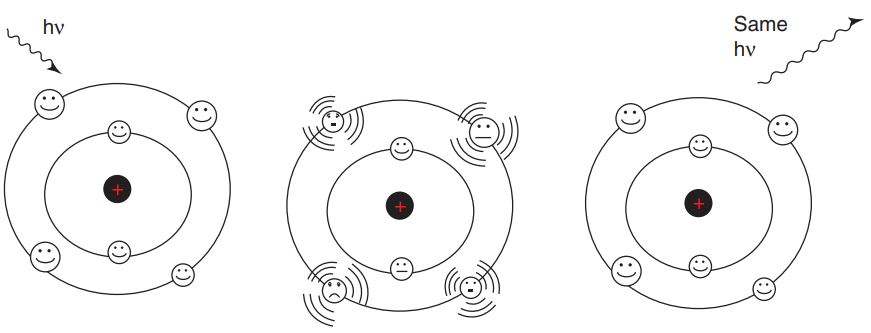
\includegraphics[width=0.5\textwidth]{Imagens/espalhamentoCoerente.JPG}
                \caption{Espalhamento Coerente}
                \label{fig:espalhamentoCoerente}
            \end{figure}

        \subsection{Efeito Fotoelétrico}

            O fóton interage com um életron fortemente ligado ao átomo do meio absorvedor, onde este fóton é totalmente absorvido e o elétron é ejetado do átomo que sai como um fóton-elétron com energia cinética igual a energia do fóton incidente subtraída da energia de ligação deste elétron ao átomo, Figura \ref{fig:efeitoFotoeletrico} , ou seja:



                \begin{equation}
                    E_k = h\nu - E_B
                \end{equation}

                \begin{figure}[h]
                    \centering
                    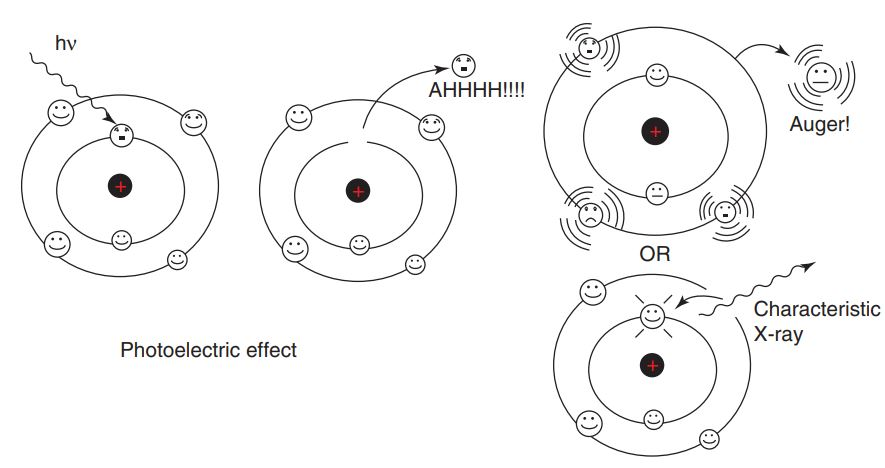
\includegraphics[width=0.6\textwidth]{Imagens/efeitoFotoeletrico.JPG}
                    \caption{Efeito Fotoelétrico}
                    \label{fig:efeitoFotoeletrico}
                \end{figure}


            \begin{itemize}
                \item O coeficiente de atenuação atômico para o efeito fótoelétrico é proporcional a: ${}_a\tau \propto Z^4 / (h\nu)^3$;
                \item o coeficiente de atenuação mássico para o efeito fotoelétrico é proporcional a
                : $\tau_m \propto (Z / h\nu)^3$
            \end{itemize}

            Conforme a energia do fóton incidente aumenta, a seção de choque mássica $\tau_m$ diminui, e existe uma descontinuidade em $\tau_m$ quando a energia do fóton incidente é igual a energia de ligação de uma das camadas internas. Esta descontinuidade é chamada de bordas de absorção e refletem o fato de que para energias do fóton incidente menores que a energia de ligação de uma determinada camada não ocorrerá o efeito enquanto que para energias maiores ou iguais o efeito ocorrerá; A Figura \ref{fig:descontinuidadeEfeitoFotoeletrico} mostra a seção de choque atômica para o efeito fotoelétrico ${}_a\tau$ para diferentes tipos de materiais em função da energia do fóton incidente, onde pode ser observado as bordas de absorção da camada K

            \begin{figure}[h]
                \centering
                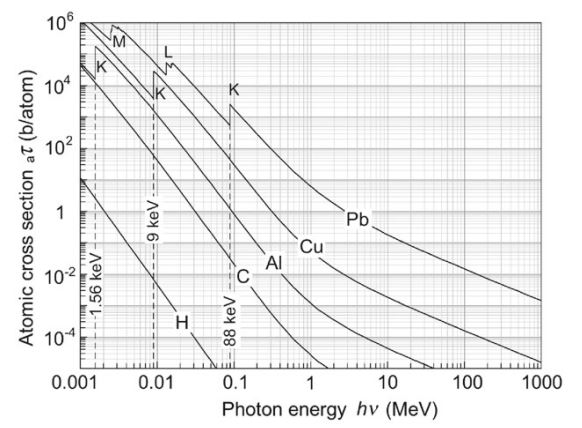
\includegraphics[width=0.6\textwidth]{Imagens/descontinuidadeEfeitoFotoeletrico.JPG}
                \caption{Efeito Fotoelétrico}
                \label{fig:descontinuidadeEfeitoFotoeletrico}
            \end{figure}

        \subsection{Espalhamento Compton}

        \subsection{Produção de Pares}

        \subsection{Produção de Tripleto}

        \subsection{Desintregação Fotonuclear}

        

\bibliography{ref.bib}
\end{document}